\documentclass[twoside]{book}
\usepackage{lectures}
\hypersetup{pdftitle={Comparison geometry}}
\makeindex

\begin{document}
\title{\tt Differential geometry\\ of curves and surfaces:\\ a working approach}
\author{\tt Anton Petrunin and Sergio Zamora Barrera}
\date{}
\maketitle
\thispagestyle{empty}

\chapter{Isoperimetric inequality}

\warning

For any plane figure $F$ with perimeter $\ell$, its area $a$ satisfies the following inequality:
\[4\pi\cdot  a \le \ell^2.\eqlbl{eq:plane-isop}\]
Moreover the equality holds if $F$ is congruent to a round disc.

This is so-called \emph{isoperimetric inequality} on the plane.
Let us reformulate it without formulas, using the comparison language.

\begin{thm}{Isoperimetric inequality}
The area of plane figure bounded by a closed curve of length $\ell$ can not exceed the area of round disc with the same circumference $\ell$.
Moreover the equality holds only if the figure is congruent to the disc.
\end{thm}

The comparison reformulation has some advantages --- it is more intuitive and it is also easier to generalize. 

\begin{thm}{Exercise} Come up with a formulation of isoperimetric inequality on the units sphere. 
Try to reformulate it as an algebraic inequality similar to \ref{eq:plane-isop}.
\end{thm}

\begin{wrapfigure}{r}{58 mm}
\vskip-4mm
\centering
\includegraphics{mppics/pic-1}
%\caption*{}
\end{wrapfigure}

Recall that a plane figure $F$ is called \index{convex figure}\emph{convex} if for every pair of points $x,y\in F$, the line segment $[x,y]$ that joins the pair of points lies also in~$F$.


The following exercise reduces the isoperimetric inequality to the case of convex figures:

\begin{thm}{Exercise}
Assume $F$ is a plane figure bounded by a closed curve of length $\ell$.
Show that there is a convex figure $F'\supset F$ bounded by a closed curve of length at most $\ell$.
\end{thm}

The following problem is named after Dido, the legendary founder and first queen of Carthage.

\begin{thm}{Dido's problem}
A figure of the maximal area bounded by a straight line and a curve of given length with endpoints on that line is a half-disc.
\end{thm}

\begin{thm}{Exercise}\label{ex:dido-isop}
Show that Dido's problem follows from the isoperimetric inequality and the other way around.
\end{thm}


\begin{thm}{Exercise}
Use the isoperimetric inequality in the plane to show that 
inscribed convex polygons have maximal area among all the polygons with the given sides.
\end{thm}

\begin{thm}{Exercise}
Find the minimal length of curve that divides the unit square in the given ratio $\alpha$.  
\end{thm}

\section{Lawlor's proof}

Here we present a sketch of the proof of Dido's problem based of the idea of Gary Lawlor in \cite{lawlor}.
Before getting into the proof, try to solve the following exercise.

{

\begin{wrapfigure}{r}{34 mm}
\vskip-4mm
\centering
\includegraphics{mppics/pic-2}
%\caption*{}
\end{wrapfigure}

\begin{thm}{Exercise}
An old man walks along a trail around a convex meadows and pulls a brick on a rope of unit length (the rope is always strained).
After walking around he noticed that the brick is at the same position as at the beginning.
Show that the area between the trail and the path of the brick equals to the area of the unit disc. 

\end{thm}

}

\parit{Sketch of the proof.}
Let $F$ be a convex figure bounded by a line and a curve $\gamma(t)$ of length $\ell$;
we can assume that $\gamma$ is a unit speed curve so the set of parameters is $[0,\ell]$.

Imagine that we are walking along the curve with a stick of length $r$ so that the other end of stick drags on the flow.
Assume that at initially (at time $t=0$) the stick points in the direction of $\gamma(\ell)$ --- the other end of $\gamma$.

\begin{wrapfigure}{r}{34 mm}
\vskip-0mm
\centering
\includegraphics{mppics/pic-3}
%\caption*{}
\bigskip
\includegraphics{mppics/pic-4}
%\caption*{}
\end{wrapfigure}

Note that is $r$ is small then most of the time we drag the stick behind. Therefore at the end of walk the stick will make more than half turn and will point to the same side of the figure.

Let $R$ be the radius of half-circle $\tilde\gamma(t)$ of length $\ell$.
Assume we walk along $\tilde\gamma$  with a stick as or length $R$ the same way as described above.
Note that the other end does not move (it always lies in the center) and the direction of stick changes with rate $\tfrac1R$.
Note further for $\gamma$ this rate would be at most $\tfrac1R$.
Therefore after walking along $\gamma$,
the stick of length $R$ will rotate at most as much as if we would walk along $\tilde\gamma$.

Hence there is a positive value $r\le R$ such that after walking along $\gamma$ the stick will rotate exactly half turn, so it will point in the direction of $\gamma(0)$.

Let us show that the area of $F$ can not exceed the area of half-disc $D$ or radius $r$;
since $r\le R$, the latter implies Dido's problem.

Imagine that stick is covered with paint and it colors the area below it while you are walking.
Notice that to color maxmimal area one has to move perpendicularly to the stick.
Therefore the total area colored after walking along $\gamma$ can not exeed the area of $D$.

It remains to show that all $F$ is colored.
Fix a point $p\in F$.
Notice that at the beginning the point $p$ lies on the left from the stick and at the end it lies on the right form it.
Therefore it will be a moment of time $t_0$ when the sides change from left to right.
At this time the point must be on the line containing the stick. Moreover if it lies on the extension then the sides change from right to left. Therefore $p$ lies on the stick; that is, $p$ is colored.
\qeds

\begin{thm}{Exercise}
Find the places with cheating in the proof above and try to fix them.
\end{thm}

\begin{thm}{Exercise} Read and understand the original proof of Gary Lawlor in \cite{lawlor}.
\end{thm}



\chapter{Length}

The material of this and the following chapters overlaps largely with \cite[Chapter 5]{fuchs-tabachnikov}.

\section{Length of curve}


\begin{thm}{Definition}\label{def:curve}
Consider a \emph{plane curve}\index{plane curve} $\alpha\:[a,b]\z\to \RR^2$;
that is $\alpha$ is a continuous mapping from the real interval $[a,b]$ to the Euclidean plane $\RR^2$. 


If $\alpha(a)=p$ and $\alpha(b)=q$,
we say that $\alpha$ is a \emph{curve from $p$ to $q$}\index{curve from $p$ to $q$}.

A curve $\alpha\:[a,b]\to \RR^2$ is called \emph{closed} if $\alpha(a)=\alpha(b)$.

A curve $\alpha$ called \emph{simple} if it is described by an injective map;
that is $\alpha(t)=\alpha(t')$ if and only if $t=t'$.
However, a closed curve $\alpha\:[a,b]\to \RR^2$ is called simple if it is injective 
everywhere except the ends; that is, if
$\alpha(t)=\alpha(t')$ for $t<t'$ then $t=a$ and $t'=b$.
\end{thm}
 
Recall that a sequence 
\[a=t_0 < t_1 < \cdots < t_k=b.\]
is called \emph{partition} of interval $[a,b]$.

\begin{thm}{Definition}\label{def:length}
Let $\alpha\:[a,b]\to \RR^2$ be a curve.
The \emph{length}\index{length of curve} of $\alpha$ is defined as

\begin{align*}
\length \alpha
= 
\sup \{|\alpha(t_0)-\alpha(t_1)|&+|\alpha(t_1)-\alpha(t_2)|+\dots
\\
&\dots+|\alpha(t_{k-1})-\alpha(t_k)|\}. 
\end{align*}

where the exact upper bound is taken over all partitions
\[a=t_0 < t_1 < \cdots < t_k=b.\]

Note that $\length\alpha\in[0,\infty]$;
the curve $\alpha$ is called \emph{rectifiable}\index{rectifiable curve} if its length is finite.
\end{thm}

Informally, one could say that the length of curve is the exact upper bound of lengths of polygonal lines \emph{inscribed} in the curve.

\begin{thm}{Exercise}
Assume $\alpha\:[a,b]\to\RR^2$ is smooth curve, in particular the velocity vector $\alpha'(t)$ is defined and depends continuously on $t$.
Show that
\[\length \alpha=\int_a^b|\alpha'(t)|\cdot dt.\]
\end{thm}

\begin{thm}{Exercise}\label{ex:nonrectifiable-curve}
Construct a nonrectifiable curve $\alpha\:[0,1]\to\RR^2$.
\end{thm}

A closed simple plane curve is called \emph{convex} if it bounds a convex figure.

\begin{thm}{Proposition}\label{prop:convex-curve}
Assume a convex figure $A$ bounded by a curve $\alpha$ lies in a figure $B$ bounded by a curve $\beta$.
Then
\[\length\alpha\le \length\beta.\]
\end{thm}

Note that it is sufficient to show that for any polygon  $P$ inscribed in $\alpha$ there is a polygon $Q$ inscribed in $\beta$ such that 
$\perim P\le \perim Q$, where $\perim P$ denotes the perimeter of $P$.

Therefore it is sufficient to prove the following lemma.


\begin{thm}{Lemma}\label{lem:perimeter}
Let $P$ and $Q$ be polygons.
Assume $P$ is convex and $Q\supset P$.
Then $\perim P\le \perim Q$.
\end{thm}


\begin{wrapfigure}{r}{24 mm}
\vskip-4mm
\centering
\includegraphics{mppics/pic-7}
%\caption*{}
\end{wrapfigure}

\parit{Proof.}
Note that by triangle inequality,
the inequality
\[\perim P\le \perim Q\]

holds
if $P$ can be obtained from $Q$ by cutting it along a chord;
that is, a line segment with ends on the boundary of $Q$ that lies in $Q$.


Note that there is an increasing sequence of polygons 
$$P=P_0\subset P_1\subset\dots\subset P_n=Q$$
such that $P_{i-1}$ obtained from $P_{i}$ by cutting along a chord.
Therefore 
\begin{align*}
\perim P=\perim P_0&\le\perim P_1\le\dots
\\
\dots&\le\perim P_n=\perim Q
\end{align*}
and the lemma follows.
\qeds

\begin{thm}{Corollary}
Any convex closed curve is rectifiable.  
\end{thm}

\parit{Proof.}
Fix a curve $\alpha\:[a,b]\to\RR^2$.
Note that $\alpha$ is bounded; indeed  

Any closed curve is bounded; that is, it lies in a sufficiently large square.


By Proposition~\ref{prop:convex-curve}, the length of the curve can not exceed the perimeter of the square, hence the result.
\qeds



\warning 
\section{Semicontinuity of length}

Recall that lower limit 
of a sequence of real numbers $(x_n)$ is denoted by
\[\liminf_{n\to\infty} x_n.\] 
It is defined as the lowest partial limit; that is a the lowest possible limit of a subsequence of $(x_n)$.
The lower limit is defined for any sequence of real numbers and it takes value in the exteded real line $[-\infty,\infty]$


\begin{thm}{Theorem}\label{thm:length-semicont}
Length is a lower semi-continuous with respect to pointwise convergence of curves. 

More precisely, assume that a sequence
of curves $\alpha_n\:[a,b]\to \RR^2$ converges pointwise 
to a curve $\alpha_\infty\:[a,b]\to \RR^2$;
that is, $\alpha_n(t)\z\to\alpha_\infty(t)$ for any fixed $t\in[a,b]$ and $n\to\infty$. 
Then 
$$\liminf_{n\to\infty} \length\alpha_n \ge \length\alpha_\infty.\eqlbl{eq:semicont-length}$$
\end{thm}



\begin{wrapfigure}{r}{20 mm}
\vskip-0mm
\centering
\includegraphics{mppics/pic-6}
\end{wrapfigure}


Note that the inequality \ref{eq:semicont-length} might be strict.
For example the diagonal of unit square $\alpha_\infty$ 

can be  approximated by a sequence of stairs-like
polygonal curves $\alpha_n$
with sides parallel to the sides of the square ($\alpha_6$ is on the picture).
In this case
\[\length\alpha_\infty=\sqrt{2}\quad
\text{and}\quad \length\alpha_n=2\]
for any $n$.

\parit{Proof.}
Fix $\eps > 0$ and choose a sequence $a=t_0<t_1<\dots<t_k=b$
such that 
\begin{align*}
\length\alpha_\infty<
|\alpha_\infty(t_0)-\alpha_\infty(t_1)|+\dots+|\alpha_\infty(t_{k-1})-\alpha_\infty(t_k)|+\eps.
\end{align*}

Set 
\begin{align*}\Sigma_n
&\df
|\alpha_n(t_0)-\alpha_n(t_1)|+\dots+|\alpha_n(t_{k-1})-\alpha_n(t_k)|.
\\
\Sigma_\infty
&\df
|\alpha_\infty(t_0)-\alpha_\infty(t_1)|+\dots+|\alpha_\infty(t_{k-1})-\alpha_\infty(t_k)|.
\end{align*}

Note that $\Sigma_n\to \Sigma_\infty$ as $n\to\infty$
and $\Sigma_n\le\length\alpha_n$ for each $n$.
Hence
$$\liminf_{n\to\infty} \length\alpha_n \ge \length\alpha_\infty-\eps.$$
Since $\eps>0$ is arbitrary, we get \ref{eq:semicont-length}.\qeds

\section{Axioms of length}

\parbf{Concatenation.}
Assume $\alpha\:[a,b]\to \RR^2$ and $\beta\:[b,c]\z\to \RR^2$ are two curves such that $\alpha(b)=\beta(b)$.
Then one can combine these two curves in one $\gamma\:[a,c]\z\to \RR^2$ by assuming that $\gamma(t)=\alpha(t)$ for $t\le b$ and $\gamma(t)\ge\beta(t)$ for $t\ge b$.
The obtained curve $\gamma$ is called the 
\emph{concatenation} of $\alpha$ and $\beta$ which can be written as $\gamma=\alpha*\beta$.

\begin{wrapfigure}{r}{30 mm}
\vskip-0mm
\centering
\includegraphics{mppics/pic-10}
\end{wrapfigure}

Note that
\[\length(\alpha*\beta)=\length\alpha+\length\beta\]
for any two curves $\alpha$ and $\beta$ such that the concatenation $\alpha*\beta$ is defined.

\parbf{Reparametrization.}
Assume $\alpha\:[a,b]\to \RR^2$ is a curve and $\tau\:[c,d]\to [a,b]$ is a continuous strictly monotonic onto map.
Consider the curve $\alpha'\:[c,d]\to \RR^2$ defined by $\alpha'=\alpha\circ\tau$.
The curves $\alpha'$ is called \emph{reparametrization} of $\alpha$.

Note that 
\[\length\alpha'=\length\alpha\]
if $\alpha'$ is a reparametrization of $\alpha$.





\begin{thm}{Proposition}\label{prop:length-axioms}
Let $\ell$ be a functional that returns a value in $[0,\infty]$ for any curve $\alpha\:[a,b]\to\RR$.

Assume it satisfies the following properties:
\begin{enumerate}[(i)]
\item\label{Normalization} (Normalization) If $\alpha\:[a,b]\to \RR^2$ is a linear curve,%
\footnote{That is $\alpha=w+v\cdot t$ for some vectors $w$ and $v$.} then
\[\ell(\alpha)=|\alpha(a)-\alpha(b)|.\]
\item\label{Additivity} (Additivity) If the concatenation $\alpha*\beta$ is defined, then
\[\ell(\alpha*\beta)=\ell(\alpha)+\ell(\beta).\]
\item\label{Motion invariance} (Motion invariance) The functional $\ell$ is invariant with respect to the motions of the plane; that is, if $m$ is a motion then 
\[\ell(m\circ\alpha)=\ell(\alpha)\]
for any curve $\alpha$.
\item\label{Reparametrization invariance} (Reparametrization invariance) If $\alpha'$ is a reparametrization of a curve $\alpha$ then
\[\ell(\alpha')=\ell(\alpha).\]
(In fact linear reparametrizations will be sufficient.)
\item\label{Semi-continuity} (Semi-continuity) If a sequence of curves $\alpha_n\:[a,b]\to \RR^2$ converges to a curve pointwise to a curve $\alpha_\infty\:[a,b]\to \RR^2$, then 
\[\liminf_{n\to\infty} \ell(\alpha_n) \ge \ell(\alpha_\infty).\]
\end{enumerate}
Then 
\[\ell(\alpha)=\length \alpha\eqlbl{eq:l=length}\] 
for any plane curve $\alpha$.

\end{thm}

\parit{Proof.}
Note that from normalization and additivity, the identity 
\[\ell(\beta)=\length \beta\eqlbl{eq:=poly}\]
holds for any polyhonal line $\beta$ that is linear on each edge.

Note that the following two inequalities 
\[\ell(\alpha)\le\length \alpha\eqlbl{eq:l<length}\]
\[\ell(\alpha)\ge\length \alpha\eqlbl{eq:l>length}\]
imply \ref{eq:l=length}; we will prove them separately. 

Fix a curve $\alpha\:[a,b]\to \RR^2$ and a partition $a=t_0\z<t_1\z<\z\dots\z<t_k=b$. 
Consider the curve $\beta\:[a,b]\to \RR^2$ defined as a linear curve from $\alpha(t_i)$ to $\alpha(t_{i+1})$  on each segment $t\in[t_i,t_j]$.
By the definition of length, 
\[\length\beta\le \length\alpha.\]

Since the map  $\alpha\:[a,b]\to \RR^2$ is continuous,
one can find a sequence of partitions of $[a,b]$ such that the corresponding curves $\beta_n$ converge to $\alpha$ pointwise.
Applying semi-continuity of $\ell$, \ref{eq:=poly} and the definition of length, we get that 
\begin{align*}
\ell(\alpha)&\le \liminf_{n\to\infty}\ell(\beta_n)=
\\
&=\liminf_{n\to\infty}\length\beta_n\le
\\
&\le\length \alpha.
\end{align*}
Hence \ref{eq:l<length} follows.

\begin{wrapfigure}{r}{36 mm}
\vskip-4mm
\centering
\includegraphics{mppics/pic-8}
\end{wrapfigure}

Note that a curve $\alpha\:[a,b]\to \RR^2$ with a partition $a=t_0\z<t_1\z<\z\dots\z<t_k=b$ can be considered as a concatenation
\[\alpha=\alpha_1*\alpha_2*\dots*\alpha_k\]
where $\alpha_i$ is the restriction of $\alpha$ to $[t_{i-1},t_i]$.

Note that there is a sequence of motions $m_i$ of the plane so that 
\[m_i\circ\alpha(t_i)=m_{i+1}\circ\alpha(t_i)\] 
for any $i$ and 
the points 
\[m_1\circ\alpha(t_0), m_1\circ\alpha(t_1),\dots m_k\circ\alpha(t_k)\] 
appear on a line in the same order.
For the concatenation 
\[\gamma=(m_1\circ\alpha_1)*(m_2\circ\alpha_2)*\dots*(m_k\circ\alpha_k)\]
we have
\[\ell(\gamma)=\ell(\alpha).\]

Note that one can find a sequence of partitions of $[a,b]$ such that reparametrizationsof  $\gamma_n$ converge to linear curve $\gamma_\infty'$;
denote these reparametrizations by $\gamma'_n$.
We can assume in addition that $\length\gamma'_\infty\z=\length\alpha$;
indeed since $\gamma'_\infty$ is linear,
\begin{align*}
\length \gamma'_\infty&=|\gamma'(a)-\gamma'(b)|=
\\
&=\lim_{n\to\infty}\Sigma_n=
\\
&=\length\alpha.
\end{align*}
where $\Sigma_n$ is the sum in the definition of length for the $n$-th partition.
Hence it is sufficient to choose a sequence of partitions such that $\Sigma_n\z\to\length\alpha$ --- by the definition of length this is possible.

Applying additivity, invariance of $\ell$ with respact to motions and reparametizations, we get that
\begin{align*}
\ell(\alpha)&=\lim_{n\to\infty}\ell(\gamma_n)=
\\
&=\lim_{n\to\infty}\ell(\gamma_n')\ge
\\
&\ge \ell(\gamma_\infty')=
\\
&=\length\alpha.
\end{align*}
Hence \ref{eq:l>length} follows.
\qeds

\begin{thm}{Exercise} 
Construct a functional $\ell$ that is different from length and satisfies all the conditions in 
 Proposition~\ref{prop:length-axioms} except the semi-continuity.
\end{thm}



\section{Crofton formula}

Let $\alpha$ be a plane curve and $u$ is a unit vector.
Denote by $\alpha_u$ the orthogonal projection of $\alpha$ to a line $\ell$ in the direction of $u$;
that is, $\alpha_u(t)\in\ell$ and $\alpha(t)-\alpha_u(t)\perp \ell$ for any $t$.

\begin{thm}{Crofton formula}
The length of any plane curve $\alpha$ is proportional to the average of lengths of its projection $\alpha_u$ for all unit vectors $u$.
Moreover for any plane curve $\alpha$ we have
\[\length\alpha=\tfrac\pi2\cdot\overline{\length \alpha_u},\]
where $\overline{\length \alpha_u}$ denotes the average value of $\length \alpha_u$.
\end{thm}

\parit{Proof.}
First let us show that the formula 
\[\length\alpha=k\cdot\overline{\length \alpha_u},\eqlbl{eq:crofton-k}\]
holds for some fixed coefficient $k$.
It will follow once we show that both sides of formula satisfies the length axioms in \ref{prop:length-axioms}.

The normalization can be acheaved by adjusting~$k$.

The semi-continuity of the right hand side follows since $\length\alpha_u$ is semi-continuous and therefore the average has to be semi-continuous.

It is straightforward to check the remaining properties.


It remains to find $k$.
Let us apply the formula \ref{eq:crofton-k} to the unit circle.
The circle has length $2\cdot\pi$ and its projection to any line has length 4 --- it is a segment of length 2 traveled back and forth.
Evidently the average value is also $4$. 
Therefore \[2\cdot \pi=k\cdot 4\]
and therefore $k=\tfrac\pi2$.
\qeds

\parbf{Reformulation via number of intersections.}
Given a pair a unit vector $u$ and a real number $\rho$,
consider the line of vectors $w$ on the plane described by the equation
\[\langle u, w\rangle =\rho,\]
where $\langle u, w\rangle$ denotes the scalar product. 
Any line on the plane admits exactly two such presentations with pair $(u,\rho)$ and $(-u,-\rho)$.
A pair $(u,\rho)$ describes uniquely an \emph{oriented} line --- that is a line with chosen unit normal vector.

Fix a unit vector $u_0$ and denote by $u(\phi)$ its rotation by angle $\phi$.
Denote by $\ell(\phi,\rho)$ the oriented line for the pair $(u(\phi),\rho)$.
To describe any line, we need a pair $(\phi,\rho)\in (-\pi,\pi]\times \RR$.

For a curve $\alpha$  set $n_\alpha(\phi,\rho)$ to be the number of parameter values $t$ such that $\alpha(t)$ lies on the line $\ell(\phi,\rho)$. 
The value $n_\alpha(\phi,\rho)$ has to be nonnegative integer or $\infty$.
Note that if $\alpha$ is simple curve then $n_\alpha(\ell)$ is the number of intersections of $\alpha$ with $\ell$.


\begin{thm}{An other Crofton formula}
For any curve $\alpha$,
\[\length\alpha=\tfrac14\cdot\iint_{(-\pi,\pi]\times \RR} n_\alpha(\rho,\phi)\cdot d\rho\cdot d\phi.\]
the integral is to be understood in the sense of Lebesgue.
\end{thm}

By definition of average value,
\[\overline{\length\alpha_u}
=
\frac1{2\cdot\pi}\cdot\int_{-\pi}^\pi \length\alpha_{u(\phi)}\cdot d\phi.\]
Therefore  proof of this reformulation of the Crofton follows from the following observation.

\begin{thm}{Observation}
If $u=u(\phi)$, then 
\[\length\alpha_u=\int_\RR n_\alpha(\rho,\phi)\cdot d\rho;\]

\end{thm}

The proof is straightforward for those who understand Lebesgue integral.

\parbf{Variations.}
The same argument can be used to derive other formulas of the same type.
For example.

Recall that big circle in a sphere is the intersection of sphere with a plane passing thru its center.
For example equator as well as any meridian are a big circles.

\begin{thm}{Spherical Crofton formula}
The length of any curve $\alpha$ in the unit sphere is $\pi$ times the average number of its crossings with big circles.

More presciently, given a unit vector $u$, denote by $n_\alpha(u)$ the number of crossings of $\alpha$ and the equator with pole at $u$.
Then 
\[\length\alpha=\overline{n_\alpha(u)}.\]

Equivalently,
\[\length\alpha=\overline{\length\alpha_u},\]
where $\alpha_u$ denotes the curve obtianed by cloasest point projection of $\alpha$ on the equator with pole at $u$.
\end{thm}


\begin{thm}{Exercise}
Come up with a Crofton formulas for curves in the Euclidean space via projections to lines and to planes.
Find the coefficients in these formulas.
\end{thm}

\section{Applications}

\parit{Alternative proof of Proposition~\ref{prop:convex-curve}.}
Note that 
\[\length \beta_u\ge \length \alpha_u\]
for any unit vector $u$.
Indeed $\alpha_u$ runs back and forth along a line segment and $\beta_u$ has to run at least as much.

It follows that 
\[\overline{\length \beta_u}\ge \overline{\length \alpha_u}.\]
It remains to apply Crofton formula.
\qeds


Recall that diameter of a plane figure $F$ is defined as the least upper bound on the distances between pairs of its points;
that is,
\[\diam F=\sup\set{|x-y|}{x,y\in F}.\]

The equilateral triangle with side 1 gives an example of convex figure of diameter 1 that can not be covered by a round disc of diameter~1.

\begin{thm}{Exercise} 
Assume $F$ is a convex figure of diameter 1 and $D$ is the round disc of diameter 1.
Show that
\[\perim F\le \perim D.\]
\end{thm}

\begin{wrapfigure}{r}{33 mm}
\vskip-5mm
\centering
\includegraphics{mppics/pic-9}
\end{wrapfigure}

A convex figure $F$ has constant width $a$ if the orthogonal projection of $F$ to any line has length $a$.
There are many non-circular shapes of constant width. 
A nontrivial example is the Reuleaux triangle shown on the picture;
it is the intersection of three round disks, each having its center on the boundary of the other two.
The following exercise is the so called Barbier's theorem.

\begin{thm}{Exercise} 
Show that figures has constant width $a$ have the same perimeter (which is equal to $\pi\cdot a$ --- the perimeter of the round disc of diameter $a$).
\end{thm}

\begin{thm}{Exercise} 
Let $\gamma$ be a closed curve in the unit sphere of length smaller than $2\cdot\pi$.
Show that $\gamma$ lies in a hemisphere.
\end{thm}

\begin{thm}{Exercise} 
Let $\alpha$ be a closed curve of length $\pi$.
Show that it lies between a pair of parallel lines on distance $1$ from each other.
\end{thm}

\begin{thm}{Exercise}
A spaceship flies around nonrotating planet or unit radius and came back to the original position;
it was able to make a picture of every point on the surface of the planet.

Try to use the Crofton formulas to get a lower bound on the length of its trajectory (does not need to be exact, but should be bigger than $2\cdot\pi$).

What do you think could be the shortest trajectory?
\end{thm}

Hausdorff distance $d_H(F,G)$ between closed bounded sets $F$ and $G$ in the plane is defined as the exact lower bound on $\eps>0$ such that $\eps$-neightborhood of $F$ contains $G$ and $\eps$-neightborhood of $G$ contains~$F$.

\begin{thm}{Exercise}
Assume $F$ and $G$ be two closed convex figures on the plane such that $d_H(F,G)<\eps$.
Show that 
\[|\perim F-\perim G|<2\cdot\pi\cdot\eps.\]

\end{thm}

The Minkowski sum of two sets $A$ and $B$ in the plane $\RR^2$ is the set denoted by $A+B$ that is formed by adding each vector in $A$ to each vector in $B$;
that is, 
\[A + B = \set{a+b}{a\in A,\ b\in B}.\]

\begin{thm}{Exercise}
Show that 
\[\perim(A+B)=\perim A+\perim B\]
for any pair of convex figures in the plane.
\end{thm}

\begin{thm}{Exercise}
Let $\gamma$ be a curve that lies in a convex figure $F$ in the plane.
Assume that
\[2\cdot \length \gamma\ge n\cdot \perim F\]
for some integer $n$.
Show that there is a line $\ell$ that has $\gamma$  at least $n$ distinct points of intersection with $\gamma$.
\end{thm}


\chapter{Curvature of curves}

\section{Total curvature}

Here we introduce the so called \emph{total curvature of curve}.
In general term \emph{curvature} is used for something that measures how 
a geometric object deviates from being a straight;
total curvature is not an exception --- as you will see if the total curvature of a curve is vanishing then the curve runs along a straight line.


Let $\alpha\:[a,b]\to\RR^3$ be a \emph{smooth} \emph{regular} curve --- smooth means that
the velocity vector $\alpha'(t)$ is defined and continuous with respect to $t$ and regular means that $\alpha'(t)\ne 0$ for any $t$.
If the curve $\alpha$ is closed then we assume in addition that $\alpha'(a)=\alpha'(b)$.

Denote by $\tau(t)$ the unit vector in the direction of $\alpha'(t)$;
that is, $\tau(t)=\tfrac{\alpha'(t)}{|\alpha'(t)|}$.
The $\tau\:[a,b]\to\mathbb{S}^2$ is an other curve which is called \emph{tangent indicatrix} of $\alpha$.
The length of $\tau$ is called \emph{total curvature of}~$\alpha$.

\begin{thm}{Exercise}
Show that the total curvature of any smooth closed regular curve $\alpha$ is at least $2\cdot\pi$.
Moreover, the equality holds if and only if $\alpha$ is a colased and conex curve that lies in a plane.
\end{thm}

\chapter{F\'ary--Milnor theorem}

\section{Tame knots}

It is tricky to make a formal definition that captures the intuitive meaning of \emph{knot}.
An attempt to define knots as simple closed curves leads to a pathological examples as the one show on the diagram --- these are so called \emph{wild knots}.
\begin{figure}[h]
\vskip-0mm
\centering
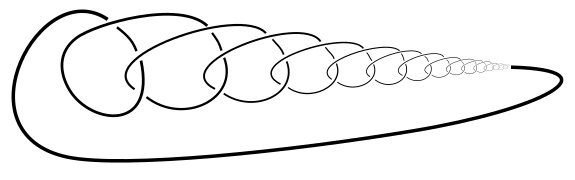
\includegraphics[scale=.6]{pics/Wild_knot}
\vskip0mm
\end{figure}
If one adds that the curve has to be smooth and regular,
then these examples disappear, but it is still a tricky to give right definition of \emph{deformation} --- the following diagram shows 
\begin{figure}[h]
\vskip-0mm
\centering

\includegraphics[scale=1]{pics/knot}
\vskip0mm
\end{figure}
that it can not be defined as a continuous family of closed simple smooth regular curves. 
Observe that all curves on the diagram are smooth and regular for all times including the last moment.

We define a \emph{knot} (more precicely \emph{tame knot}) as a simple closed polygonal line in Euclidean space~$\RR^3$.

The notation $\triangle abc$ is used for triangle $abc$; that is a polygonal line with three edges and vertexes $a$, $b$ and $c$.
Let us denote by $\solidtriangle abc$ the convex hull of the points $a$, $b$ and $c$; $\solidtriangle abc$ is the solid triangle with the vertexes $a$, $b$ and $c$.
The points $a$, $b$ and $c$ are assumed to be distinct, but they might lie on one line;
that is, for us a degenerate triangle is a triangle.

We understand a \emph{triangular isotopy} of a knot to be the generation of a new knot from the original one by means of the
following two operations:

Assume $[pq]$ is an edge of the knot and $x$
is a point such that the solid triangle $\solidtriangle pqx$  has no common points with the knot except for the edge $[pq]$.
Then we can replace the edge $[pq]$ in the knot by two adjacent edges $[px]$ and $[xq]$.

We can also perform the inverse operation.
That is, if for two adjacent edges $[px]$ and $[xq]$ of a knot the triangle
$\solidtriangle pqx$ has no common points with the knot except for the points on the edges $[px]$ and $[xq]$,
then we can replace two adjacent edges $[px]$ and $[xq]$ by one edge $[pq]$.

Polygons that arise from one another by a finite sequence of
triangular isotopies are called \emph{isotopic}.

\begin{wrapfigure}{r}{25 mm}
\vskip-0mm
\centering
\includegraphics{mppics/pic-18}
\vskip0mm
\end{wrapfigure}

A knot that is not isotopic to a triangle is called nontrivial.

The trefoil knot shown on the diagram gives a simple example of nontrivial knot.
A proof that the trefoil knot is nontrivial can be found in any textbook on knot theory, we do not give it here.
The most elementary and visual proof is based on the so called \emph{tricolorability} of knot diagrams.   

\begin{thm}{Exercise}\label{ex:triangle-isotopy}
Let $x$ and $y$ be two points on the adjacent edges $[p_1p_2]$ and $[p_2p_3]$ of a knot $\beta=p_1p_2p_3\dots p_n$.
Assume that the solid triangle $\solidtriangle xp_2y$ intersects $\beta$ only along the $[xp_2]\cup [p_2y]$.
Show that the knot $\beta'=p_1xyp_3\dots p_n$ is isotopic to $\beta$.
\end{thm}



\section{F\'ary--Milnor theorem}

We will give few proofs of the following theorem.

\begin{thm}{Theorem}\label{thm:fary-milnor}
The total curvature of any nontrival knot is at least $4\cdot\pi$. 
\end{thm}

The famous F\'ary--Milnor theorem states that the inequality is strict;
that is, the total curvature of any nontrival knot \emph{exceeds} $4\cdot\pi$.
It is easy to construct a trefoil knot with total curvature arbitrary close to $4\cdot\pi$;
therefore this result is optimal.

The question was raised by Karol Borsuk \cite{borsuk} and answered independently by Istv\'an F\'ary and John Milnor \cite{fary, milnor};
latter few other proofs were found.

\section{Milnor's proof}

In the proof we will use the following fact. 

\begin{thm}{Proposition}\label{prop:one-max-one-min}
Assume that a height function $(x,y,z)\to z$ 
has only one local minimum and one local maximum on a closed simple polygonal line and all the vertexes of the polygonal line lie on different height.
Then the line is a trivial knot.
\end{thm}

The proof is a simple application of the definition of isotopy, given in the previous section. 

\begin{wrapfigure}{r}{20 mm}
\vskip-0mm
\centering
\includegraphics{mppics/pic-19}
\vskip0mm
\end{wrapfigure}

\parit{Proof.}
Let $\beta=p_1\dots p_n$ be the closed simple polygonal line
such that the height function $(x,y,z)\to z$ has one local minimum one local maximum.
Note that on each of the two arcs of $\beta$ from min-vertex to max-vertex the height function increases monotonically.

Consider three vertexes with the largest value of the height function;
they have to include the max-vertex and two more.
Note that these three vertexes are consequent in the polygonal line; 
without loss of generality we can assume that they are $p_{n-1},p_n,p_1$.

Note that the solid triangle $\solidtriangle p_{n-1}p_np_1$ does not intersect any edge $\beta$ except the two adjacent edges $[p_{n-1}p_n]\cup[p_np_1]$.
Indeed, if $\solidtriangle p_{n-1}p_np_1$ intersects $[p_1p_2]$,
then, 
since $p_2$ lies below $\solidtriangle p_{n-1}p_np_1$,
$[p_1p_2]$ must intersect $[p_{n-1}p_n]$
which is impossible since $\beta$ is simple.
The same way one can show that $\solidtriangle p_{n-1}p_np_1$ can not intersect $[p_{n-2}p_{n-1}]$.
The remaining edges lie below $\solidtriangle p_{n-1}p_np_1$, hence they can not intersect this triangle.

Applying triangular isotopy, to $\solidtriangle p_{n-1}p_np_1$ we get a closed simple polygonal line $\beta'\z=p_1\dots p_{n-1}$ which is isotopic to $\beta$.

Since all the vertexes $p_i$ have different height,
the assumption of proposition holds for $\beta'$.

Repeating this procedure $n-3$ times we get a triangle.
Hence $\beta$ is a trivial knot.
\qeds

\parit{Milnor's proof of \ref{thm:fary-milnor}.}
Let $\alpha$ be a simple closed polygonal line.
Assume its total curvature is less that $4\cdot\pi$.
Then by Proposition~\ref{prop:tc-crofton}, 
\[\tc\alpha_u<4\cdot\pi\]
for some unit vector $u$.
Moreover, we can assume that $u$ points in a generic direction;
that is, $u$ is not perpendicular to any edge or diagonal of $\alpha$.

The total curvature of $\alpha_u$ is $\pi$ times the number of turns of $\alpha_u$
which has to be an even number.
It follows that number of turns of $\alpha_u$ is at most $2$;
it can not be less than 2 for generic direction and therefore it is $2$.

That is, if we rotate the space so that $u$ pints to the top,
than the height function has exactly one minimum and one maximum;
by Proposition~\ref{prop:one-max-one-min}, $\alpha$ is a trivial knot --- hence the result.
\qeds

\section{F\'ary's proof}

Let us give a sketch of another proof, based on the original idea of Istv\'an F\'ary.

\begin{wrapfigure}{r}{30 mm}
\vskip-0mm
\centering
\includegraphics{mppics/pic-13}
\vskip0mm
\end{wrapfigure}

\parit{F\'ary's proof of \ref{thm:fary-milnor}.}
Consider a projection of the knot to a plane in general position.
That is, we assume that the self-intersections of the projection are at most double and the projection of each edge does not degenerate.
The obtained closed polygonal line $\beta=p_1p_2\dots p_n$ divides the plane into domains, one of which is unbounded, denote it by $U$, and the others are bounded.

First note that all domains can be colored in a chessboard order;
that is, they can be colored in black and white in such a way that domains with common borderline get different colors.
If the unbounded domain gets white color and every other domain is black then one can untie the knot by flipping these domains one by one.

\begin{thm}{Exercise}
Give a formal proof of the last statement; that is, show that if only undbounded domain is white then $\beta$ is isotopic to a triangle. 
\end{thm}

\begin{wrapfigure}{r}{30 mm}
\vskip-4mm
\centering
\includegraphics{mppics/pic-14}
\vskip0mm
\end{wrapfigure}

Therefore among the bounded domains there is a white domain, denote it by $D$.
The domain $D$ can not have a borderline with $U$ since they have the same color.
Fix a point $o$ in this domain.

For each $i$, set 
\begin{align*}
\phi_i&=\pi-\measuredangle p_{i-1}p_ip_{i+1},
\\
\psi_i&=\measuredangle p_{i-1} o p_{i},
\\
\theta_i&=\measuredangle o p_i p_{i+1}.
\end{align*}
Here indexes are taken modulo $n$; in particular, $p_{n}=p_0$.


Note that $\phi_i$ is the external angle at $p_i$;
therefore 
\[\tc\beta= \phi_1+\dots+\phi_n\]

Direct calculations show that 
\[\phi_i\ge \psi_i+\theta_{i-1}-\theta_i.\]
In the two pictures below, $\phi_i$ is the solid angle;
the rest of angles $\psi_i$, $\theta_{i-1}$ and $\theta_i$
are the same.
We have equality on the first picture and strict inequality on the second picture.

\begin{figure}[h]
\vskip-0mm
\centering
\includegraphics{mppics/pic-15}
\vskip0mm
\end{figure}

It follows that 
\[\phi_1+\dots+\phi_n\ge \psi_1+\dots+\psi_n.\]

The last sum 
is the total angle at  which $\beta$ seen from $o$ counted with multiplicity. 
The boundary of $D$ contributes at least $2\cdot\pi$ to this sum and the boundary of $U$ contributes an other $2\cdot\pi$;
since their boundaries do not overlap we get 
\[\psi_1+\dots+\psi_n\ge 4\cdot\pi,\]
hence the result.

This is true for the projection of the knot to any plane in general position.
The remaining planes contribute nothing to the average value.
Therefore by Proposition~\ref{prop:tc-crofton}, the total curvature of the original knot is at least $4\cdot\pi$.
\qeds



\begin{thm}{Exercise}
Construct a closed smooth simple curve with total curvature arbitrary close to $2\cdot\pi$ such that its projection to any plane has at least $10$ self-intersections.   
\end{thm}



\section{Proof of Alexander and Bishop}

Here we sketch a proof of F\'ary--Milnor theorem given by of Stephanie Alexander and Richard Bishop in \cite{alexander-bishop}.

The proof is elementary, but not simple 
(elementary does not mean simple, it means only that it does not use much theory).
It is based on the following two facts that we already familiar with:
\begin{itemize}
\item If a closed polygonal line $\beta'$ is inscribed in a closed polygonal line $\beta$ then 
 \[\tc\beta'\le \tc\beta.\]
\item The total curvature of doubly covered
bigon is $4\cdot\pi$; that is,
\[\tc\beta=4\cdot\pi\]
if $\beta=pqpq$ for two distinct points $p$ and $q$.
Similarly if a quadrilateral is sufficiently close to a doubly covered
bigon, then its total curvature is close to $4\cdot\pi$.
\end{itemize}


\parit{Proof.}
Let $\beta=p_1\dots p_n$ be a closed polygonal line that is not a trivial knot;
that is, one can not get a triangle from $\beta$ by applying a sequence of triangular isotopys defined in the previous section.

We proceed by induction on the number $n \ge 3$.
In the base case $n=3$ the polygonal line $\beta$ is a triangle.
Therefore, by the definition, $\beta$ is a trivial knot --- nothing to prove.

Consider the smallest $n$ for which the statement fail;
that is, there is a closed simple polygonal line $\beta\z=p_1\dots p_n$ that is not a trivial knot such that
\[\tc\beta<4\cdot\pi.
\eqlbl{eq:<4pi}\]
We use the indexes modulo $n$ that is $p_0=p_n$, $p_1=p_{n+1}$ and so on.
Without loss of generality, we may assume that $\beta$ is in general position; 
that is, no four vertexes of $\beta$ lie on one plane. 

Set $\beta_0=\beta$.
If the solid triangle $\solidtriangle p_{0}p_1p_{2}$ intersects $\beta_0$ only by the two adjacent edges,
then applying the corresponding triangular isotopy, we get a knot $\beta'_0$ with $n-1$ edge that is inscribed in $\beta_0$ therefore
\[\tc\beta_0\ge \tc\beta_0'.\]
On the other hand by induction hypothesis 
\[\tc\beta_0'\ge 4\cdot\pi\]
which contradicts \ref{eq:<4pi}.

Choose the first point $w'_1$ on the edge $[p_1p_2]$ so that the line segment $[p_0w'_1]$ 
intersects $\beta_0$.
Denote a point of intersection by $y_1$.

\begin{wrapfigure}{r}{25 mm}
\vskip-0mm
\centering
\includegraphics{mppics/pic-17}
\vskip0mm
\end{wrapfigure}

Choose a point $w_1$ on $[p_1p_2]$ a bit before $w'_1$
(below we explain how close).
Denote by $x_1$ the point on $[p_0w_1]$ that minimize the distance to $y_1$.
This way we get a closed polygonal line 
$\beta_1\z=w_1p_2\dots p_n$ with two marked points $x_1$ and $y_1$.
Denote by $m_1$ the number of edges in the arc $y_1w_1\dots x_1$ of $\beta_1$.

By Exercise~\ref{ex:triangle-isotopy}, $\beta_1$ is isotopic to $\beta_0$;
in particular $\beta_1$ is a nontrivial knot.

Now let us repeat the procedure for the adjacent edges $[w_1b_2]$ and $[b_2b_3]$ of $\beta_1$.
If the solid triangle $\solidtriangle w_1b_2b_3$ intersects $\beta_1$ only at these two adjacent edges, then we get a contradiction with the induction hypothesis the same way as before.
Otherwise we get a new knot $\beta_2=w_1w_2b_3\dots b_n$ with two marked points $x_2$ and $y_2$.
Denote by $m_2$ the number of edges in the broken line $y_2w_3\dots x_2$.

Note that the points $x_1,x_2,y_1,y_2$ can not appear on $\beta_2$ in the same cyclic order;
otherwise the broken line $x_1x_2y_1y_2$ can be made to be arbitrary close to a doubly covered bigon which again contradicts~\ref{eq:<4pi}.%
\footnote{More precisely, the choice of $w_1$ has to be made so that the distance $|x_1-y_1|$ would be much less that all the distances between $y_1$ and any point $z\in\beta\cap \solidtriangle p_1p_2p_3$, so we have
\[\measuredangle y_1zx_1<\tfrac\eps{10},\]
where $\eps=4\cdot\pi-\tc\beta$.
In this case, since $y_2\in \beta\cap \solidtriangle p_1p_2p_3$ and $x_2$ can be taken arbitrary close to $y_2$, we have
\[\tc x_1x_2y_1y_2 > 4\cdot\pi -\eps= \tc\beta\]
which can not happen since $x_1x_2y_1y_2$ is inscribed in $\beta$.}

Therefore we can assume that the arc $x_2w_2\dots y_2$ lies inside of arc $x_1w_1\dots y_1$ in $\beta_2$
and therefore $m_1>m_2$.

Continuing this procedure we get a sequence of polygonal lines $\beta_i\z=w_1\dots w_i p_{i+1}p_n$ with marked points $x_i$ and $y_i$ such that the number of edges $m_i$ from $x_i$ to $y_i$ decreases in $i$.
Clearly $m_i>1$ for any $i$ and $m_1<n$.
Therefore it requires less than $n$ steps we get a contradiction with the induction hypothesis.
\qeds

\begin{wrapfigure}{r}{30 mm}
\vskip-0mm
\centering
\includegraphics{mppics/pic-20}
\vskip0mm
\end{wrapfigure}

\begin{thm}{Exercise}
Suppose that a closed curve $\alpha$ crosses a line at four points $a$, $b$, $c$ and $d$.
Assume that the points $a$, $b$, $c$ and $d$ appear on the line in the same order and they appear on the curve $\alpha$ in the order $a$, $c$, $b$, $d$.
Show that 
\[\tc\alpha\ge 4\cdot\pi.\]
\end{thm}

A line crossing a knot at four points as in the exercise is called \emph{alternating quadrisecants}.
It turns out that any nontrivial knot adits an alternating quadrisecants \cite{denne};
it provides yet an other proof of F\'ary--Milnor theorem.


\begin{thm}{Advanced exercise}
Show that given any real number $\Phi$ there is a knot $\beta$ such that any knot isotopic to $\beta$ has total curvature at least~$\Phi$.   
\end{thm}

\parit{Hint:} Use that there are knots with arbitrary large \emph{bridge number}, see for example \cite{schultens} and the references there in.



\chapter{Osculating circlines}


\section{Acceleration of unit-speed curve}

Any regular smooth curve can be parametrized by its length.
The obtained curve $\alpha$ (that is the constructed reparametrization of the given curve) has unit speed; 
that is, $|\alpha'(t)|=1$ for any $t$.
A curve with such parametrization is called \emph{unit-speed} curve
or a curve with a \emph{natural parametrization}. 

It is straightforward to show any smooth regular curve remains smooth (and surely regular) if equipped with a natural parametrization; 
here smooth means that all derivatives $\alpha^{(n)}(t)$ are defined for any $n$ and all values of $t$ in the domain of definition of $\alpha$.

\begin{thm}{Proposition}\label{prop:a'-pertp-a''}
Assume $\alpha\:[a,b]\to\RR^2$ be a smooth unit-speed curve.
Then 
\[\alpha'(t)\perp \alpha''(t)\]
for any $t$.
\end{thm}

The scalar product (also known as dot product) of two vectors $v$ and $w$ will be denoted by $\langle v,w\rangle$.
Recall that for derivative of scalar product the product rule holds;
that is if $v=v(t)$ and $w=w(t)$ are smooth vector-valued functions of real argument $t$, then
\[\langle v,w\rangle'=\langle v',w\rangle+\langle v,w'\rangle.\]

\parit{Proof.}
Since $|\alpha'(t)|=1$, we have
\[\langle\alpha'(t),\alpha'(t)\rangle=1.\]
Taking derivative of both sides we get
\[2\cdot\langle\alpha''(t),\alpha'(t)\rangle=0,\]
hence the result.
\qeds

\section{Signed curvature}

Given a vector $v\in \RR^2$ denote by $i\cdot v$ the vector obtained from $v$ by the counterclockwise rotation by $\tfrac\pi2$.
(The ``multiplication'' by $i$ agrees with the miultiplication by imaginary unit if one use  complex coordinates on the plane $z=x+i\cdot y$.)

Suppose $\alpha\:[a,b]\to\RR^2$ is a smooth unit-speed curve.
Recall that curvature of $\alpha$ at $t$ can be defined as $|\alpha''(t)|$.

The \emph{signed curvature} $\kappa_\alpha(t)$ is uniquely defined by
the identity 
\[\alpha''(t)=\kappa_\alpha(t)\cdot i\cdot \alpha'(t).\]
Note that by Proposition~\ref{prop:a'-pertp-a''} this equation has a solution.
Since $|\alpha'(t)|=1$ we have that $|\kappa_\alpha(t)|=|\alpha''(t)|$ for any $t$.

The signed curvature measures how fast the direction $\tau(t)=\alpha'(t)$ rotates;
if is positive if it turns left and negative if it turns right;
if the curve goes straight then its curvature vanish.

\section{Osculating circline}

It is straightforward to prove the following statement.

\begin{thm}{Proposition}\label{prop:circline}
Given a point $p$,
a unit vector $u$ 
and a real number $\kappa$ there is unique smooth unit-speed curve $\gamma\:\RR\to\RR^2$ 
that starts at $p$ in the direction of $u$ and has constant signed curvature $\kappa$.

Moreover if $\kappa=0$, then $\gamma$ runs along a line $\gamma=p+t\cdot u$
and if $\kappa\ne 0$, then $\gamma$ runs around a circle of radius $\tfrac1{|\kappa|}$ with center at $p+\tfrac i\kappa\cdot u$. 
\end{thm}

Further we will use term \emph{circline} for \emph{circle or line}.

{

\begin{wrapfigure}{r}{30 mm}
\vskip-4mm
\centering
\includegraphics{mppics/pic-21}
\vskip0mm
\end{wrapfigure}

\begin{thm}{Definition}
Let $\alpha$ be a smooth unit-speed plane curve;
denote by $\kappa_\alpha(t)$ the signed curvature of $\alpha$ at $t$.

A unit-speed plane curve $\gamma$ of constant signed curvature $\kappa_\alpha(t_0)$ that starts at $\alpha(t_0)$ and runs in the direction $\alpha'(t_0)$ is called \emph{osculating circline} of $\alpha$ at $t_0$.
\end{thm}

}

The center and radius of the osculating circle at a given point are called \emph{center of curvature} and \emph{radius of curvature} of the curve at that point.

\section
{Spiral theorem}
\label{spiral}

The following theorem states that 
if you drive on the plane and turn the steering wheel to the right all the time,
then you will not be able to come back to the same place.
This theorem was proved by Peter Tait \cite[see][]{tait}
and later rediscovered by Adolf Kneser \cite[see][]{kneser}.

\begin{thm}{Theorem}\label{thm:spiral}
Assume $\alpha$ is a smooth regular plane curve with strictly monotonic curvature. 
Then $\alpha$ is simple.
\end{thm}

The same statement holds for signed curvature; the proof requires only minor modifications.

\begin{thm}{Exercise}
Show that a 3-dimensional analog of the theorem does not hold.
That is, there are self-intersecting smooth regular space curves with strictly monotonic curvature.
\end{thm}


The proof of theorem is based on the following lemma.

\begin{thm}{Lemma}
Assume that $\alpha$ is a smooth regular plane curve with strictly decreasing positive signed curvature. Then the osculating circles of $\alpha$ are nested; that is, if $\gamma_t$ denoted the osculating circle of $\alpha$ at $t$,
then $\gamma_{t_0}$ lies in the open disc bounded by $\gamma_{t_1}$ for any $t_0<t_1$. 
\end{thm}

The osculating circles of the curve $\alpha$ give a peculiar foliation of an annulus by circles; it has the following property: if a smooth function is constant on each osculating circle it must be constant in the annulus \cite[see][Lecture 10]{fuchs-tabachnikov}.
Also not the the cure $\alpha$ is tangent to the circle of the foliation at each of its point, however it does not run along a circle.



\begin{wrapfigure}{o}{25 mm}
\begin{lpic}[t(-4 mm),b(-2 mm),r(0 mm),l(0 mm)]{pics/kneser-log(1)}
\end{lpic}
\end{wrapfigure}



\parit{Proof.}
Let $z(t)$ be curvature center
and 
\[r(t)=\tfrac1{\kappa_\alpha(t)}\]
is radius of curvature of $\alpha$ at $t$.
Note that 
\[z(t)=\alpha(t)+r(t)\cdot i\cdot \alpha'(t).\]
Therefore
\begin{align*}
z'(t)&=\alpha'(t)+r'(t)\cdot i\cdot \alpha'(t)+r(t)\cdot i\cdot \alpha''(t)=
\\
&=\alpha'(t)+r'(t)\cdot i\cdot \alpha'(t)+r(t)\cdot i\cdot \kappa_\alpha(t)\cdot i\cdot\alpha'(t)=
\\
&=\alpha'(t)+r'(t)\cdot i\cdot \alpha'(t)-\alpha'(t)=
\\
&=r'(t)\cdot i\cdot \alpha'(t).
\end{align*}
Since $\kappa_\alpha(t)$ is decreasing, $r(t)$ is increasing;
therefore $r'\ge 0$.
It follows that $|z'(t)|= r'(t)$ and $z'(t)\perp\alpha'(t)$.

Note that the curve $z(t)$ does not have straight arcs;
therefore
\[
\begin{aligned}
|z(t_1)-z(t_0)|&<\int_{t_0}^{t_1}|z'(t)|\cdot dt=
\\
&=\int_{t_0}^{t_1}r'(t)\cdot dt=
\\
&=r(t_1)-r(t_0).
\end{aligned}
\leqno({*})
\]

By $({*})$, the osculating circle at $t_0$ lies inside of the osculating circle at $t_1$ without touching it.
\qeds

\parit{Proof of \ref{thm:spiral}.}
Note that $\alpha(t)\in \gamma_t$ for any $t$.
Applying the lemma we get
$\alpha(t_1)\ne \alpha(t_0)$ if $t_1\ne t_0$.
Hence the result.\qeds

The lemma can be used to solve the following exercise.

\begin{thm}{Exercise}\label{ex:double-tangent}
Assume that $\alpha$ is a smooth regular plane curve with strictly monotonic curvature.
\begin{enumerate}[(a)]
\item\label{ex:double-tangent:a}Show that no line can be tangent to $\alpha$ at two distinct points.
\item Show that no circle can be tangent to $\alpha$ at three distinct points. 
\end{enumerate}
\end{thm} %???monotone or monotonic???

\begin{wrapfigure}{r}{35 mm}
\vskip-0mm
\centering
\includegraphics{mppics/pic-25}
\vskip0mm
\end{wrapfigure}

Note that part (\ref{ex:double-tangent:a}) does not hold for smooth regular plane curve with strictly monotonic \emph{signed} curvature; an example is shown on the diagram.





\chapter{Supporting circlines}

\section{Definitions}

Suppose $\alpha\:[a,b]\to\RR^2$ is a smooth unit-speed plane curve and $t_0\z\in(a,b)$.

\begin{wrapfigure}{r}{43 mm}
\vskip-4mm
\centering
\includegraphics{mppics/pic-28}
\vskip0mm
\end{wrapfigure}

A circline $\gamma$ supports $\alpha$ at $t_0$ if $\alpha(t_0)\in\gamma$
and $\gamma$ lies locally on one side of $\alpha$.
If $p=\gamma(t_0)$ for a single value $t_0$,
then we can also say \emph{$\gamma$ supports $\alpha$ at $p$} without ambiguity.

More precisely, assume that there is a round neighborhood $U\ni p$ such that for some interval $[a',b']\ni t_0$
the arc $\bar\alpha=\alpha|_{[a',b']}$ has no self-intersection and runs from boundary to boundary of $U$.
In this case $\alpha$ divides $U$ intosets  $L$ and $R$;
$L$ lies on the left and $R$ lies on the right from~$\bar\alpha$.
If $\gamma\cap U$ contains only points of $\bar\alpha$ and $R$, we say that \emph{$\gamma$ supports $\alpha$ on the right};
if $\gamma\cap U$ contains only points of $\bar\alpha$ and $L$, we say that \emph{$\gamma$ supports $\alpha$ on the left}.



Note that a circle supports itself on the right and left at the same time.

Suppose a unit-speed circline $\gamma$ supports a smooth unit-speed plane curve $\alpha$ at $t_0$.
Without loss of generality we can assume that $\gamma(0)\z=\alpha(t_0)$. 
Then $\gamma'(0)=\pm\alpha'(t_0)$.
If not, then the curve $\alpha$ would cross $\gamma$ transversely and therefore could not stay on the same side for values close to $t_0$.
Therefore reverting the parametrization of $\gamma$ if necessary we may (and further will) assume that 
\[\gamma'(0)=\alpha'(t_0)\]
holds for any supporting circline $\gamma$ to $\alpha$ at $t_0$.

\section{Supporting test}

The following proposition resembles the second derivative test. 

\begin{thm}{Proposition}\label{prop:supporting-circline}
Assume $\gamma$ is a circle that that supports $\alpha$ at $t_0$ from the rigth (correspondingly left).  
Then 
\[\kappa(t_0)\ge \kappa
\quad(\text{correspondingly}\quad\kappa(t_0)\le \kappa).
\] 
where $\kappa$ is the signed curvature of $\gamma$ 
and $\kappa(t_0)$ is the signed curvature of $\alpha$ at $t_0$.

A partial converse also holds.
Namely, suppose a unit-speed circline $\gamma$ with signed curvature $\kappa$ starts at $\alpha(t_0)$ in the direction $\alpha'(t_0)$.
Then $\gamma$ supports $\alpha$ at $t_0$ from the right (correspondingly left) if 
\[\kappa(t_0)> \kappa
\quad(\text{correspondingly}\quad\kappa(t_0)< \kappa).
\]

\end{thm}

\parit{Proof.}
We prove only the case $\kappa>0$.
The 2 remaining cases $\kappa=0$ and $\kappa<0$ can be done essentially the same way.

Since $\kappa\ne0$, the curve $\gamma$ is a circle.
According to Proposition~\ref{prop:circline},
$\gamma$ has radius $\tfrac1\kappa$ and it is centered at 
\[z=\alpha(t_0)+\tfrac i\kappa\cdot \alpha'(t_0).\]
Consider the function 
\[f(t)=|z-\alpha(t)|^2-\tfrac1{\kappa^2}.\]

Note that $f(t)\le0$ (correspondingly $f(t)\ge0$) 
if an only if $\alpha(t)$ lies on the closed left (correspondingly right) side from $\gamma$.
It follows that 
\begin{itemize}
\item if $\gamma$ supports $\alpha$ at $t_0$ from the right, 
then
\[f'(t_0)=0\quad\text{and}\quad f''(t_0)\le 0;\]

\item if $\gamma$ supports $\alpha$ at $t_0$ from  the left, 
then 
\[f'(t_0)=0\quad\text{and}\quad f''(t_0)\ge 0;\]

\item if 
\[f'(t_0)=0\quad\text{and}\quad f''(t_0)< 0,\]
then $\gamma$ supports $\alpha$ at $t_0$ from  the right;

\item if 
\[f'(t_0)=0\quad\text{and}\quad f''(t_0)> 0,\] then $\gamma$ supports $\alpha$ at $t_0$ from  the left;
\end{itemize}

Direct calculations show that
\begin{align*}
f(t_0)&=0;
\\
f'(t_0)&=\left.\langle z-\alpha(t),z-\alpha(t) \rangle'\right|_{t=t_0}=
\\
&=-2\cdot \langle \alpha'(t_0),z-\alpha(t_0) \rangle=
\\&=-2\cdot \langle \alpha'(t_0),\tfrac i\kappa \cdot\alpha'(t_0) \rangle=
\\
&=0;
\\
f''(t_0)&=\langle z-\alpha(t),z-\alpha(t) \rangle''|_{t=t_0}=
\\
&=2\cdot\left( \langle \alpha'(t_0),\alpha'(t) \rangle-\langle \alpha''(t_0),z-\alpha(t) \rangle \right)=
\\
&=2\cdot\left(1-\kappa\cdot \frac1{\kappa(t_0)}\right)
\end{align*}
Hence the result.\qeds


\begin{thm}{Exercise}
Assume $\alpha$ is a closed smooth unit-speed plane curve that runs in a unit disk.
Show that there is a point on $\alpha$ with curvature at least $1$.

Give two proofs, one based on the DNA inequality \ref{thm:DNA} and another one based on Proposition~\ref{prop:supporting-circline}.
\end{thm}

\begin{thm}{Exercise}
Assume a closed smooth regular plane curve $\alpha$ runs between parallel lines on distance 1 from each other.
Show that there is a point on $\alpha$ with curvature at least $1$.
\end{thm}


\section{Lens lemma}

\begin{thm}{Lemma}\label{lem:lens}
Let $\alpha$ be a smooth regular simple curve that runs from $x$ to $y$.
Assume that $\alpha$ runs on the right side (correspondingly left side) of the oriented line $xy$ and only its end points $x$ and $y$ lie on the line.
Then $\alpha$ has a point with positive  (correspondingly negative) curvature.
\end{thm}

\begin{wrapfigure}{r}{35 mm}
\vskip-4mm
\centering
\includegraphics{mppics/pic-22}
\vskip0mm
\end{wrapfigure}

Note that the lemma fails for curves with self-intersections;
the curve $\alpha$ on the diagram always turns right, 
so it has negative curvature everywhere, but it lies on the right side of the line $xy$. 

\parit{Proof.}
Choose points $p$ and $q$ on $\ell$
so that the points $p, x, y, q$ appear in the same order on $\ell$.

Consider the smallest disc segment with chord $[pq]$ that contains $\alpha$.
Note that its arc $\gamma$ supports $\alpha$ at a point $s=\alpha(t_0)$.

\begin{wrapfigure}{R}{50 mm}
\centering
\includegraphics{mppics/pic-23}
\bigskip
\includegraphics{mppics/pic-24}
\vskip0mm
\end{wrapfigure}

Note that the $\alpha'(t_0)$ is tangent to $\gamma$ at $s$.
Moreover $\alpha'(t_0)$ points in the direction of $q$;
that is, if we go along $\gamma$ in the direction  of $\alpha'(t_0)$ then we have to start at $p$ and end at $q$.
If the direction is opposite, then the arc of $\alpha$ from $s$ to $y$ would be trapped in the curvelinear triangle $xsp$ bounded by arcs of $\gamma$, $\alpha$ and the line segment $[px]$.
But this is impossible since $y$ does not belong to this triangle.



It follows that $\gamma$ supports $\alpha$ at $t_0$ from the right.
By Proposition~\ref{prop:supporting-circline}, 
\[\kappa(t_0)\ge \kappa,\]
where $\kappa(t_0)$ is signed curvature of $\alpha$ at $t_0$ and $\kappa$ is the curvature of $\gamma$.
Evidently $\kappa>0$, hence the result.
\qeds

\section{Convexity and inflection points}

\begin{thm}{Exercise}
Assume $\alpha$ is a closed regular simple plane curve with positive signed curvature.
Show that $\alpha$ bounds a convex set.%
\footnote{Hint: show that any tangent line to $\alpha$ is supporting.}
\end{thm}

\begin{thm}{Exercise}\label{ex:convex+2pi}
Assume $\alpha$ is a closed smooth regular plane curve with positive signed curvature.
Show that $\alpha$ is simple if and only if its total curvature is $2\cdot\pi$. 
\end{thm}


\begin{thm}{Exercise}\label{ex:1-supporting} Assume a smooth regular curve $\alpha$ has curvature at most $1$ at any point (that is, $|\kappa_\alpha(t)|\le 1$ for any $t$).
Show that both unit circles tangent to $\gamma$ at $t_0$ are supporting.

Moreover, there is $\eps>0$ ($\eps=\tfrac12$ will do) such that any arc of $\alpha$ of length $<\eps$ starting at $p=\alpha(t_0)$ cannot enter the unit circle tangent to $\alpha$ at $p$.  
\end{thm}


\begin{thm}{Exercise}
Suppose $\alpha$ is a simple smooth regular curve in the plane with positive curvature.
Assume $\alpha$ crosses a line $\ell$ at the points $p_1,p_2,\dots p_n$ and these points appear on $\alpha$ in that same order.
\begin{enumerate}[(a)]

\item Show that $p_2$ can not lie between $p_1$ and $p_3$ on $\ell$.

\item Show that if $p_3$ lies between $p_1$ and $p_2$ on $\ell$ then they appear on $\ell$ in the following order:  
\[p_1,p_3,\dots,p_4 ,p_2.\]

\item Try to describe all possible orders when $p_1$ lies between $p_2$ and $p_3$ (see the diagram).

\end{enumerate}
\end{thm}

\begin{figure}[h!]
\vskip-0mm
\centering
\includegraphics{mppics/pic-29}
\vskip0mm
\end{figure}

Recall that $\Conv X$ denotes the convex hull of the set $X$;
that is, $\Conv X$ is the intersection of all convex sets containing $X$.

\begin{thm}{Exercise}\label{ex:convex-hull}
Suppose $\alpha$ is a simple smooth regular curve with positive curvature in the plane.
Then the boundary of $\Conv \alpha$ is formed by an arc of $\alpha$ together with a line segmet connecting the ends of this arc.
\end{thm}

\begin{thm}{Exercise}
Suppose $\alpha$ is a simple smooth regular curve in the plane.
Show that $\alpha$ lies on one side from one of its tangent lines. 
\end{thm}

If the curvature of a curve $\alpha$ vanishes at $t_0$, then we say that $t_0$ is inflection value of the parameter, and $p=\alpha(t_0)$ is an inflection point;
the later convention might be ambiguous only if $\alpha$ has a self-intersection at $p$. 
In other words, $t_0$ is an inflection value if the osculating circline at $t_0$ coincides with the tangent line. 

\begin{figure}[h!]%{r}{30 mm}
\centering
\includegraphics{mppics/pic-30}
\vskip0mm
\end{figure}

\begin{thm}{Exercise}
Let $\alpha\:\RR\to\RR^2$ be a smooth simple regular plane curve.
Assume $\alpha$ is periodic in the following sense:
there is $T>0$ and a vector $v\in\RR^2$ such that 
\[\alpha(t+T)=\alpha(t)+v.\]
Show that $\alpha$ has at least 2 inflection points in the interval $[0,T]$.

\end{thm}

\begin{thm}{Theorem} 
Let $\alpha$ be a closed simple smooth regular plane curve.
Assume $\alpha$ has exactly two inflection points dividing $\alpha$ in two arcs $\alpha_1$ and $\alpha_2$.
Then 
\[\Conv \alpha_1\supset \alpha_2
\quad\text{or}\quad
\Conv \alpha_2\supset \alpha_1.\]

\end{thm}

\parit{Proof.}
Let us denote the inflection points by $v$ and $w$
and orient the arcs $\alpha_1$ and $\alpha_2$ from $v$ to $w$; we can then assume that both arcs $\alpha_1$ and $\alpha_2$ have positive curvature.

Set $F=\Conv \alpha_1$.
By Exercise~\ref{ex:convex-hull}, $F$ is bounded by an arc $\bar\alpha_1$ of $\alpha_1$ from $x$ to $y$ 
and the line segment $xy$.
We may assume that the line $xy$ is horizontal, $x$ lies on the left from $y$ and so $\alpha_1$ lies below the line.

\begin{figure}[h!]
\vskip-0mm
\centering
\includegraphics{mppics/pic-31}
\vskip0mm
\end{figure}

If $F\not\supset \alpha_2$, then $\alpha_2$ runs outside of $F$, so it has to cross the line segment $xy$.
Denote by $p_1, p_2,\dots$ the points of intersection of $\alpha_2$ with the line $xy$ as they appear on $\alpha_2$.

Since $\alpha_2$ has positive curvature, $p_1$ lies on left from $p_0$.
If $p_2$ lies between $x$ and $p_1$ then the curve $\alpha_2$ is trapped in the region bounded by the arc $xvp_2$ of $\alpha$ and the line segment $p_2x$;
therefore it can not reach $w$ --- a contradiction.
Therefore $p_2$ lies on the extension of $yx$ behind $x$.

Further $p_3$ lies on right from $p_2$. 
If $p_3$ lies between $p_1$ and $x$, then $\alpha_2$ is trapped in the region bounded by the arc $xvp_3$ of $\alpha$ and the line segment $p_3x$ --- a contradiction again.
Therefore $p_3$ lies on the extension of $xy$ behind $y$ and the arc $p_2p3$ of $\alpha$ surrounds $F$.
Whence
\[\Conv \alpha_2\supset \alpha_1.\]
\qedsf


\section{Four-vertex theorem}

A vertex of a smooth regular curve is defined as a critical point of its curvature;
in particular, any local minimum (or maximum) of the curvature is a vertex.

\begin{thm}{Exercise}\label{ex:vert-support}
Assume the osculating circle of a curve $\alpha$ at $t_0$ supports $\alpha$ at $t_0$.
Show that $t_0$ is a vertex of $\alpha$.
\end{thm}

\begin{thm}{Four-vertex theorem}\label{thm:4-vert}
Any smooth regular simple plane curve has at least four
vertices.
\end{thm}

\begin{wrapfigure}{o}{20 mm}
\vskip-0mm
\centering
\includegraphics{mppics/pic-26}
\vskip0mm
\end{wrapfigure}

Evidently any closed curve has at least two vertexes --- where the minimum and the maximum of the curvature are attained.
On the diagram the vertexes are marked;
the first curve has one self-intersection and exactly two vertexes;
he second curve has exactly four vertexes and no self-intersections.

The four-vertex theorem was first proved by Syamadas Mukhopadhyaya \cite{mukhopadhyaya} for convex curves.
By now it has a large number of different proofs and generalizations.
We will present a proof given by Robert Osserman \cite{osserman}.

\parit{Proof.}
Fix a simple smooth regular closed plane curve $\alpha$.

Suppose that $2\cdot n$ points $p_1,s_1,\dots,p_n,s_n$ appear on a closed curve $\alpha$ in the same cyclic order.
Fix a real number $\kappa$.
Assume that the curvature of $\alpha$ at $p_i$ is at least $\kappa$ and its curvature at $s_i$ is at most $\kappa$.
Then each of $n$ arcs $p_{n}p_1$, $p_{1}p_2, \dots p_{n-1}p_n$ of
$\alpha$ has a point of minimum curvature in its interior.
Similarly each of the $n$ arcs $s_{n}s_1$, $s_{1}s_2, \dots s_{n-1}s_n$ of
$\alpha$ has a point of maximum curvature.

If one of these local minima coincides with a local maximum,
an arc around this point has constant curvature;
in this case all these points are vertexes and we have an infinite number of them.
If they are all different, then we have at least $2\cdot n$ vertexes.

Therefore it is sufficient to show that

\begin{clm}{}\label{clm-key}
there are at least 4 points $p_1,s_1,p_2,s_2$ with the described properties for some $\kappa$.
\end{clm}


Note that
\begin{clm}{}\label{clm:circumscribed circle}
$\alpha$
admits a unique \emph{circumscribed circle} $\gamma$; that is, a circle of minimal radius that encloses $\alpha$.
\end{clm}

Denote by $r$ the infimum of radii of circles that enclose $\alpha$.
We can choose a sequence of circles $\gamma_n$ enclosing $\alpha$ such that their radii $r_n\to r$.
Note that all the centers of $\gamma_i$ lie at a bounded distance from $\alpha$.
Therefore passing to a subsequence we can assume that the centers of $\gamma_n$ converge to a point $o$.
Note that the circle $\gamma$ with center $o$ and radius $r$ encloses $\alpha$;
hence the existence of the circumscribed circle follows.

If there are two distinct circumscribed circles, then $\alpha$ lies in the intersection of the discs bounded by these circles.
But this intersection is enclosed in a circle of smaller radius --- a contradiction.
Hence Claim \ref{clm:circumscribed circle} follows.


\begin{clm}{}
Assume $\gamma$ is the circumscribed circle of $\alpha$.
Then $\gamma$ touches $\alpha$ at least $2$ points which divide the $\gamma$ in arcs no longer than a semicircle.
\end{clm}

\begin{wrapfigure}{r}{38 mm}
\vskip-4mm
\centering
\includegraphics{mppics/pic-271}
\vskip0mm
\end{wrapfigure}


If it was not the case, then one could move $\gamma$ slightly keeping its radius the same so that $\gamma$ will not touch $\alpha$ at all.
But in this case $\alpha$ could be enclosed in a circle of smaller radius --- a contradiction.


Let us orient $\alpha$ and $\gamma$ counterclockwise.
Then at the common points the directions of $\alpha$ and $\gamma$ coincide.
Note that these points appear on $\alpha$ and $\gamma$ in the same order;
otherwise $\alpha$ would not be simple.

Denote by $\kappa$ the signed curvature of $\gamma$, since it is oriented counterclockwise,
$\kappa\z=\tfrac1r>0$.

\begin{wrapfigure}{R}{38 mm}
\vskip-0mm
\centering
\includegraphics{mppics/pic-27}
\vskip0mm
\end{wrapfigure}
  
Fix two common points $p_1$ and $p_2$ of $\alpha$ and $\gamma$.
By Proposition~\ref{prop:supporting-circline}, the curvature of $\alpha$ at $p_1$ and $p_2$ is at least $\kappa$.
Let $\bar\alpha$ be the arc of $\alpha$ from $p_1$ to $p_2$.

We can assume that the circle is centered at the origin 
and the points $p_1$ and $p_2$ lie on the same vertical line in the right halfplane of the coordinate plane.

Let $o$ be the center of $\gamma$.
Consider another circle $\gamma'$ with the same radius $r$ and center $o'$ the leftmost point in the $x$-axis such that $\gamma^{\prime}$ intersects $\bar\alpha$.

Denote by $s_1$ a common point of $\bar\alpha$ and $\gamma'$;
we can assume that $s_1$ is not an end point of $\bar\alpha$.
At the point $s_1$ the directions of $\bar\alpha$ and $\gamma'$ coincide,
otherwise $\alpha$ could not be simple --- the same argument is used in the proof of Lemma~\ref{lem:lens}.
Therefore $\gamma'$ supports $\alpha$ from the left at $s_1$.
By Proposition~\ref{prop:supporting-circline}, the curvature of $\alpha$ at $s_1$ is at most $\kappa$.

Repeating the same argument for another pair of points $p_2,p_3$,\footnote{If $p_1$ and $p_2$ divide $\gamma$ into two semicircles, then we can take $p_3=p_1$.} 
we prove Claim \ref{clm-key}.
Hence the theorem follows.
\qeds

\begin{thm}{Exercise}
Show that any smooth regular curve of constant width has at least 6 vertexes.
\end{thm}

\section{Moon in a puddle}

\begin{thm}{Exercise}\label{ex:moon}
Let $F$ be a convex plane figure bounded by a simple closed smooth regular curve $\alpha$ of curvature bounded by 1.
Assume $\alpha$ is oriented counterclockwise, so the figure $F$ lies on the left from $\alpha$.
Show that there is a unit circle that is globally supporting $\alpha$ form the left at any given point.
\end{thm}

The following theorem was proved by Vladimir Ionin and German Pestov \cite{pestov-ionin}.
It gives a first nontrivial example of the so called ``local to global theorems'' --- based on some local data (in this case the curvature of a curve) we can conclude a global property (in this case existence of a large disc surrounded by the curve).
For convex curves, the result was known much earlier \cite[\S 24]{blaschke}.

\begin{thm}{Theorem}\label{thm:moon}
Assume $\alpha$ is a simple closed smooth regular plane curve of curvature bounded by 1.
Then it surrounds a unit disc.
\end{thm}

\parit{Proof.}
Denote by $F$ the closed region surrounded by $\alpha$. 

\begin{figure}[h!]%{r}{38 mm}
\vskip-0mm
\centering
\includegraphics{mppics/pic-32}
\vskip0mm
\end{figure}

Fix $p_1\in \alpha$.
Consider the disc $D_1$ of maximal radius 
that is tangent to $\alpha$ at $p_1$ and lies completely in $F$.

If the radius of $D_1$ is at least $1$, then the problem is solved.
Otherwise note that $p_1$ is an isolated point of the intersection $D_p\cap \alpha$.
Moreover according to Exercise~\ref{ex:1-supporting}, there is a fixed value $\eps>0$ such that any arc of $\alpha$
that starts at $p_1$ can not end in $D_1$.


Consider an arc $\alpha_1$ of $\alpha$ that runs along $\alpha$ from $p_1$ to the next point in $D_1$.
Denote by $F_1$ the region that contains $D_1$ and whose boundary is formed by $\alpha_1$ and part of the boundary of $D_1$.
From above $\length \alpha_1>\eps$.

Let $p_2$ be the midpoint of $\alpha_1$.
Let $D_2$ be the disc of maximal radius that is tangent to $\alpha_1$ at $p_2$ and lies completely in $F_1$. 
The disc $D_2$ touches the boundary $\partial F_1$ at other points, dividing it in at least two arcs.

Note that $D_2$ can not touch the boundary of $D_1$, otherwise it would lie inside $D_1$, which is impossible.
Therefore at least one of these arcs, say $\alpha_2$, do not contain the common boundary of $F_1$ and $D_1$.
Note that 
\[\length \alpha_2< \tfrac12\cdot\length\alpha_1.\]

Again, if the radius of $D_2$ is at least $1$, then the theorem is proved.
By Exercise~\ref{ex:1-supporting}, it happens if $\length \alpha_2<\eps$.
If the radius is less than 1, denote by $F_2$ the region that contains $D_2$ and is bounded by $\alpha_2$ and a part of the boundary of $D_2$. Clearly, we can repeat this construction as many times as needed. 

Since the length of the arc gets at least twice as small on each step, 
after several steps the obtained disc $D_n$ will lie completely in $F_{n-1}$ and therefore in $F$. 
\qeds

A straightforward modification of the above proof gives the following.

\begin{thm}{Theorem}\label{thm:moon+4-vert}
Suppose $\alpha$ is a closed simple smooth regular plane curve.
Denote by $F$ and $G$ the two closed domains bounded by $\alpha$, say $F$ is bounded and $G$ is unbounded.  
Then $\alpha$ has at least 2 osculating circlines that lie in $F$
and  2 osculating circlines that lie in $G$. 
\end{thm}

Note that Theorem~\ref{thm:moon} as well as the Four-vertex theorem \label{thm:4-vert} follow from Theorem~\ref{thm:moon+4-vert};
the first implication is evident and the second follows from Exercise~\ref{ex:vert-support}.



%cf. W. Blaschke, Kreis und Kugel, see pp. 115–116, Veit, Leipzig, 1916; S. B. Jackson, Bull. Amer. Math. Soc. 50 (1944), 564–578; MR0010992; G. Pestov and V. Ionin, Dokl. Akad. Nauk SSSR 127 (1959), 1170–1172; MR0107214; the reviewer, Geom. Dedicata 12 (1982), no. 4, 371–381; MR0672867

\chapter{Surfaces}
\section{Embedded surfaces}

Recall that a function $f$ of two variables $x$ and $y$ is called \emph{smooth} if all its partial derivatives $\frac{\partial^{m+n}}{\partial x^m\partial y^n}f$ are defined and are continuous in the domain of definition of $f$. 

A subset $\Sigma \subset \mathbb{R}^3$ is called a \emph{smooth surface} (or more precisely \emph{smooth regular embedded surface}) if it can be described locally as a graph of a smooth function in an appropriate coordinate system.

More precisely, any point $p\in \Sigma$ admits a neighborhood $U$ such that
in some coordinate system $(x,y,z)$, 
the intersection $W=U\cap \Sigma$ can be written as a graph $z=f(x,y)$ of a smooth function $f$ defined in an open domain of the $(x,y)$-plane.

Once we get a local representation of the surface by a graph, we can change it using the Proposition~\ref{prop:perp} below.

\parbf{Examples.}
The simplest example of a surface is the $(x,y)$-plane 
\[\Pi=\set{(x,y,z)\in\RR^3}{z=0}.\]
The plane $\Pi$ is a surface since
it can be described as the graph of the function $f(x,y)=0$.

All other planes are surfaces as well since one can choose a coordinate system so that it becomes the $(x,y)$-plane.
We can also present a plane as a graph of a linear function 
$f(x,y)=a\cdot x+b\cdot y+c$ for some constants $a$, $b$ and $c$
if the plane is not perpendicular to the $(x,y)$-plane.

A more interesting example is the unit sphere 
\[\SS^2=\set{(x,y,z)\in\RR^3}{x^2+y^2+z^2=1}.\]
This set is not the graph of any function,
but $\SS^2$
can be covered by 6 graphs 
\begin{align*}
z&=f_\pm(x,y)=\pm \sqrt{1-x^2-y^2},
\\
y&=g_\pm(x,z)=\pm \sqrt{1-x^2-z^2},
\\
x&=h_\pm(y,z)=\pm \sqrt{1-y^2-z^2};
\end{align*}
each function $f_\pm,g_\pm,h_\pm$ is defined in an open unit disc.
Therefore the unit sphere is a smooth surface.

\parbf{More conventions.}
If the surface $\Sigma$ is compact, then it is called \emph{closed surface} (the term \emph{closed set} is not directly relevant).

If $\Sigma$ is closed and noncompact, then it is called  \emph{open surface} (again the term \emph{open set} is not relevant).
For example, paraboloids 
\[z=x^2+y^2\quad\text{or}\quad z=x^2-y^2\]
are open surfaces, while the
open disc in a plane 
\[\set{(x,y,z)\in\RR^3}{x^2+y^2<1, z=0}\]
is a surface which is not an open surface since the set is not closed. 

A closed subset in a surface that is bounded by one or more smooth curves is called \emph{surface with boundary}; in this case the collection of curves is called the \emph{boundary line} of the surface.
When we say \emph{surface} we usually mean a surface without boundary;
we may use the term \emph{surface with possibly nonempty boundary} if we need to talk about surfaces with and without boundary.

\section{Tangent plane}

Let $z=f(x,y)$ be a local graph realization of a surface. 
Assume $p=(x_p,y_p,z_p)$ lies on this graph, so $z_p=f(x_p,y_p)$.
The plane passing thru $p$ and spanned by the vectors $(\tfrac{\partial}{\partial x}f)(x_p,y_p)$ and  $(\tfrac{\partial}{\partial y}f)(x_p,y_p)$ is called the \emph{tangent plane} of $\Sigma$ at $p$.
It can be interpreted as the best approximation of the surface $\Sigma$ by a plane at $p$.

The tangent plane to $\Sigma$ at $p$ is usually denoted by $\T_p$ or $\T_p\Sigma$.

It is straightforward to check that the tangent plane does not depend of the local presentation of $\Sigma$ by a graph.

\parbf{On local graph representations.}
The following proposition guarantees the existence of a local graph representation near a given point.

\begin{thm}{Proposition}\label{prop:perp}
Assume the tangent of a smooth surface $\Sigma$ at point $p$ is not perpendicular to the $(x,y)$-plane.
Then a neighborhood of $p$ in $\Sigma$ can be presented as a graph of smooth function $z=f(x,y)$ defined on an open set of the $(x,y)$-plane.
\end{thm}

A reader familiar with the inverse function theorem, can consider this proposition as an exercise.

\parbf{Special coordinate system.}
Fix a point $p$ in a smooth surface $\Sigma$.
Consider a coordinate system $(x,y,z)$ with origin at $p$ such that the $(x,y)$-plane coincides with $\T_p$.

According to Proposition~\ref{prop:perp}, 
we can present $\Sigma$ locally around $p$ as a graph of a function $f$.
Note that $f$ satisfies the following additional properties:
\begin{align*}
f(0,0)&=0,
&
(\tfrac{\partial}{\partial x}f)(0,0)&=0,
&
(\tfrac{\partial}{\partial y}f)(0,0)&=0.
\end{align*}
The first equality holds since $p=(0,0,0)$ lies on the graph and the last two equalities mean that the tangent plane at $p$ is horizontal.

This gives an almost canonical coordinate system in a neighborhood of $p$;
it is unique up to a rotation of  the $(x,y)$-plane and switching the sign of the $z$-coordinate.

\section{Curvatures}

\parbf{Hessian.}
Fix a point $p$ on a smooth surface $\Sigma$ and the associated special coordinate system. 

Consider the Hessian matrix 
\[M_p=\begin{pmatrix}
   (\tfrac{\partial^2}{\partial x^2}f)(0,0)
   &(\tfrac{\partial^2}{\partial x\partial y}f)(0,0)
   \\
   (\tfrac{\partial^2}{\partial y\partial x}f)(0,0)
   &(\tfrac{\partial^2}{\partial y^2}f)(0,0)
  \end{pmatrix}.
\]
This is a symmetric matrix, therefore by an appropriate rotation of the $(x,y)$-plane, we can make it diagonal;
that is, we can assume that $(\tfrac{\partial^2}{\partial x\partial y}f)(0,0)=0$.
Then the diagonal elements are called \emph{principle curvatures} of $\Sigma$ at $p$;
they are uniqueley defined up to sign;
They are denoted as $k_1(p)$ and $k_2(p)$.
The principle curvatures can be also defined as the eigenvalues of $M_p$.

The determinant of $M_p$ is $k_1(p)\cdot k_2(p)$;
it is called the \emph{Gauss curvature} of $\Sigma$ at $p$.
The trace of $M_p$ is $k_1(p)+ k_2(p)$;
it is called the \emph{mean curvature} of $\Sigma$ at $p$.

Form the discussion above, 
we get that the Gauss curvature depends only on $\Sigma$ and $p$,
and not on the choice of the coordinate system.
Up to sign, the same obsevation is true for the principle curvatures and the mean curvature. 


\begin{thm}{Exercise}\label{ex:projection}
Assume $\Sigma$ is a closed surface of with principle curvatures at most 1
and let $F$ be its orthogonal projection to a plane.
Show that no circle of curvature larger than 1 can support $F$ from the left. 
\end{thm}

\begin{thm}{Exercise}
Show that any closed immersed surface has a point with positive Gauss curvature.
\end{thm}

\begin{thm}{Exercise}
Assume a closed surface $\Sigma$ bounds a convex body.
Show that $\Sigma$ is a sphere with nonnegative Gauss curvature. 
\end{thm}

\section{Immersed surfaces}

\parbf{Parametrizations.}
A surface can be described by a map from a known surface to the space.
For example the ellipsoid
\[\Sigma_{a,b,c}=\set{(x,y,z)\in\RR^3}{\tfrac{x^2}{a^2}+\tfrac{y^2}{b^2}+\tfrac{z^2}{c^2}=1}\]
for some positive numbers $a,b,c$ can be defined as the image of the map $s\:\SS^2\to\RR^3$, defined as the restriction of the map $(x,y,z)\mapsto (a\cdot x, b\cdot y,c\cdot z)$ to the unit sphere $\SS^2$.

For a surface $\Sigma$, a map $s: \Sigma \to \RR ^3$ is called a 
\emph{parametrized surface} if it is smooth and regular in the sense defined below. 
$\Sigma$ will be called the \emph{domain of parameters} and $s$ the \emph{parametrization}.

Assume $\Sigma$ is written locally as a graph $z=f(x,y)$ in some coordinate system. Let $\tilde{f} $ be defined on the same domain as $f$ as $\tilde{f}(x,y) = (x,y, f(x,y))$.

The map $s\:\Sigma \to \RR^3$ is  smooth if for the composition $s\circ \tilde{f}$, all partial derivatives $\frac{\partial^{m+n}}{\partial x^m\partial y^n}(s\circ \tilde{f})$ exist and are continuous in the domain of definition of $f$.

The map $s\:\Sigma \to \RR^3$ is regular
if the vectors $\frac{\partial}{\partial x}(s\circ \tilde{f})$ and $\frac{\partial}{\partial y}(s\circ \tilde{f})$ are linearly independent at each point of the domain of $f$.

Evidently the parametric definition includes the embedded surfaces defined previously --- as the domain of parameters we can take the surface itself and the identity map as $s$.

\parbf{Immersed surfaces.} The parametric definition allows the surfaces to have self-intersections, hence it is more general.
The surfaces with possible self-intersections are  called \emph{immersed}.

In the described example $\SS^2$ is the \emph{domain of parameters} of the surface.
We can say that the surface $\Sigma_{a,b,c}$ is a \emph{sphere} since it has the sphere as the domain of parameters.

We may use other domains of parameters, the torus or the sphere with two handles or for surfaces with boundary, the disc, the annulus, the M\"obius band and so on.
The sphere with $n$ handles is also called the \emph{surface of genus $n$}.

The set of parameters can be more complicated, for example the projective plane --- a sphere where opposite points are identified; such set of parameters can not be realized as an embedded surface in $\RR^3$, but it can be embedded in a higher dimensional Euclidean space.
Another example is the Klein bottle --- the  nonoriented brother of the torus;
it also can not be embedded in the Euclidean space, but it can be immersed with a self-intersection along a closed smooth curve.











\section{Curves in a surface}\label{sec:Darboux}

\begin{wrapfigure}{o}{42 mm}
\vskip-4mm
\centering
\begin{lpic}[t(-0mm),b(0mm),r(0mm),l(0mm)]{asy/paraboloid+curve(1)}
\lbl[ul]{34,14;$\tan$}
\lbl[b]{20,43;$\Norm$}
\lbl[bl]{38,35;$\mu$}
\end{lpic}
\vskip-0mm
\end{wrapfigure}

Suppose $\gamma$ is a regular smooth curve in a smooth oriented surface $\Sigma$.
As usual we denote by $\Norm$ the unit normal field on~$\Sigma$.

Without loss of generality we may assume that $\gamma$ is unit-speed;
in this case $\tan(s)=\gamma'(s)$ is its tangent indicatrix.
Let us use the shortcut notation $\Norm(s)\z=\Norm(\gamma(s))$.
Note that the unit vectors $\tan(s)$ and $\Norm(s)$ are orthogonal.
Тherefore there is a unique unit vector $\mu(s)$\index{10tmn@$\tan$, $\mu$, $\Norm$} such that 
$\tan(s),\mu(s),\Norm(s)$ is an oriented orthonormal basis;
it is called the \index{Darboux frame}\emph{Darboux frame} of $\gamma$ in $\Sigma$.
Since $\T_{\gamma (s)}\z\perp\nu(s)$, the vector $\mu(s)$ is tangent to $\Sigma$ at $\gamma(s)$.
In fact $\mu(s)$ is a counterclockwise rotation of $\tan(s)$ by the angle $\tfrac\pi2$ in the tangent plane $\T_{\gamma(s)}$.
This vector can also be defined as the vector product $\mu(s)=\nu(s)\times \tan(s)$.

Since $\gamma$ is unit-speed, we have that $\gamma''\perp \gamma'$ (see \ref{prop:a'-pertp-a''}).
Therefore the acceleration of $\gamma$ can be written as a linear combination of $\mu$ and $\Norm$;
that is,
\[\gamma''(s)=k_g(s)\cdot \mu(s)+k_n(s)\cdot\Norm(s).\]\index{10k@$k_g$, $k_n$}
The values $k_g(s)$ and $k_n(s)$ are called \index{geodesic curvature}\emph{geodesic} and \index{normal curvature}\emph{normal curvatures} of $\gamma$ at $s$, respectively.
Since the frame $\tan(s),\mu(s),\nu(s)$ is orthonormal, these curvatures can be also written as the following scalar products:
\begin{align*}
k_g(s)&=\langle \gamma''(s),\mu(s)\rangle
=
\\
&=\langle \tan'(s),\mu(s)\rangle.
\\
k_n(s)&=\langle \gamma''(s),\Norm(s)\rangle=
\\
&=\langle \tan'(s),\Norm(s)\rangle.
\end{align*}

Since $0=\langle \tan(s),\Norm(s)\rangle$ we have 
that 
\begin{align*}
0&=\langle \tan(s),\Norm(s)\rangle=
\\
&=\langle \tan'(s),\Norm(s)\rangle+\langle \tan(s),\Norm'(s)\rangle=
\\
&=k_n(s)+\langle \tan(s),D_{\tan(s)}\nu\rangle.
\end{align*}
Applying the definition of shape operator,
we get the following:

\begin{thm}{Proposition}\label{prop:normal-shape}
Assume $\gamma$ is a smooth unit-speed curve in a smooth surface $\Sigma$.
Let $p=\gamma(s_0)$ and $\vec v=\gamma'(s_0)$.
Then 
\[k_n(s_0)=\langle \Shape_p(\vec v),\vec v\rangle,\]
where $k_n$ denotes the normal curvature of $\gamma$ at $s_0$ and $\Shape_p$ is the shape operator at $p$.
\end{thm}

Note that according to the proposition, the normal curvature of a regular smooth curve in $\Sigma$ is completely determined by the velocity vector $\vec v$ at the point $p$.
By that reason the normal curvature is also denoted by $k_{\vec v}$;\index{10k@$k_{\vec v}$}
according to the proposition,
\[k_{\vec v}=\langle \Shape_p(\vec v),\vec v\rangle\]
for any unit vector $\vec v$ in $\T_p$.

Let $p$ be a point on a smooth surface $\Sigma$.
Assume we choose tangent-normal coordinates at $p$ so that the Hessian matrix is diagonalized, then we have
\[M_p=\begin{pmatrix}
   k_1(p)
   &0
   \\
   0
   &k_2(p)
  \end{pmatrix}.
\]
Consider a vector ${\vec w}=(\begin{smallmatrix}a\\b
\end{smallmatrix})$ in the $(x,y)$-plane.
Then
\begin{align*}
\langle \Shape(\vec w),\vec w\rangle
&=\langle M_p\cdot(\begin{smallmatrix}a\\b
\end{smallmatrix}),(\begin{smallmatrix}a\\b
\end{smallmatrix})\rangle=
\\
&=a^2\cdot k_1(p) +b^2\cdot k_2(p). 
\end{align*}
If ${\vec w}$ is unit, then $a^2+b^2=1$ which implies the following:

\begin{thm}{Observation}\label{obs:k1-k2}
For any point $p$ on an oriented smooth surface $\Sigma$,
the principle curvatures $k_1(p)$ and $k_2(p)$ are respectively the minimum and maximum of the normal curvatures at $p$.
Moreover, if $\theta$ is the angle between a unit vector ${\vec w}\in\T_p$ and the first principle direction at $p$, then 
\[k_{\vec w}(p)=k_1(p)\cdot(\cos\theta)^2+k_2(p)\cdot(\sin\theta)^2.\]

\end{thm}

The last identity is called \index{Euler's formula}\emph{Euler's formula}.

\begin{thm}{Exercise}\label{ex:mean-curvature}
Let  $\Sigma$ be a smooth surface.
Show that the sum of the normal curvatures for any pair of orthogonal directions, at a point $p\in\Sigma$ equals $H(p)$ --- the mean curvature at $p$. 
\end{thm}




\begin{thm}{Meusnier's theorem}\label{thm:meusnier}
Let $\gamma$ be a regular smooth curve that runs along a smooth oriented surface $\Sigma$.
Let $p=\gamma(t_0)$, ${\vec v}\z=\gamma'(t_0)$, and $\alpha=\measuredangle(\Norm(p),\norm(t_0))$;
that is, $\alpha$ is the angle between the unit normal to $\Sigma$ at $p$ and the unit normal vector in the Frenet frame of $\gamma$ at~$t_0$.
Then the following identity holds true 
\[\kur(t_0)\cdot\cos\alpha=k_{n}(t_0);\]
here $\kur(t_0)$  and $k_n(t_0)$ are the curvature and the normal curvature of $\gamma$ at $t_0$, respectively.  
\end{thm}


\parit{Proof.} Since $\gamma''=\tan'=\kur\cdot \norm$, we get that
\begin{align*}
k_{n}(t_0)&=\langle\gamma'',\Norm\rangle=
\\
&=\kur(t_0)\cdot\langle\norm,\Norm\rangle=
\\
&=\kur(t_0)\cdot\cos\alpha.
\end{align*}
\qedsf

The theorem above, as well as the statement in the following exercise were proved by Jean Baptiste Meusnier \cite{meusnier}.

\begin{thm}{Exercise}\label{ex:meusnier}
Let $\Sigma$ be a smooth surface, $p\in\Sigma$ and ${\vec v}\in \T_p\Sigma$ a unit vector.
Assume that $k_{\vec v}(p)\ne 0$; that is, the normal curvature of $\Sigma$ at $p$ in the direction of ${\vec v}$ does not vanish.

Show that the osculating circles at $p$ of smooth regular curves in $\Sigma$ that run in the direction ${\vec v}$ sweep out a sphere $S$ with center $p+\tfrac1{k_{\vec v}}\cdot\Norm$ and radius $r=\tfrac1{|k_{\vec v}|}$.
\end{thm}

\begin{thm}{Exercise}\label{ex:principle-revolution}
Let $\gamma(s)=(x(s),y(s))$ be a smooth unit-speed simple plane curve in the upper half-plane,
and  $\Sigma$ be the surface of revolution around the $x$-axis with generatrix $\gamma$.

\begin{enumerate}[(a)]
\item Show that the parallels and meridians are lines of curvature on $\Sigma$.
\item Show that 
\[\frac{|x'(s)|}{y(s)}
\quad
\text{and}
\quad
\frac{-y''(s)}{|x'(s)|}
\]
are the principle curvatures of $\Sigma$ at $(x(s),y(s),0)$ in the direction of the corresponding parallel and meridian respectively.
\item Show that $\Sigma$ has Gauss curvature $-1$ at all points if and only if $y$ satisfies the following differential equation.
\[y''=y.\] 
The case  $y=e^{-s}$ --- the so-called \emph{psudosphere}; is shown on the diagram.
\end{enumerate}

\end{thm}

\begin{figure}[h!]
\vskip-7mm
\hskip20mm
\includegraphics{asy/pseudosphere}
\vskip-3mm
\end{figure}

\begin{thm}{Exercise}\label{ex:catenoid-is-minimal}
Show that the \index{catenoid}\emph{catenoid} defined implicitly by the equation
\[(\cosh z)^2=x^2+y^2\]
is a minimal surface.
\end{thm}

\begin{thm}{Exercise}\label{ex:helicoid-is-minimal}
Show that the \index{helicoid}\emph{helicoid} defined by the following parametric equation
\[s(u,v)=(u\cdot \sin v,u\cdot \cos v,v)\]
is a minimal surface.
\end{thm}

\section{Lagunov's example}

\begin{thm}{Exercise}\label{ex:moon-revolution}
Assume $V$ is a body in $\RR^3$ bounded by a smooth surface of revolution with principle curvatures at most 1 in absolute value.
Show that $V$ contains a unit ball.
\end{thm}

The following question is a 3-dimensional analog of the moon in a puddle problem (\ref{thm:moon}).

\begin{thm}{Question}\label{quest:lagunov}
Assume a set $V\subset \RR^3$ is bounded by a closed connected surface $\Sigma$ with 
principle curvatures bounded in absolute value by 1.
Is it true that $V$ contains a ball of radius 1?
\end{thm}

According to \ref{ex:moon-revolution}, the answer is ``yes'' for surfaces of revolution.
Latter (see \ref{ex:convex-lagunov})
we will show that the answer is ``yes'' for convex surfaces.
Now we are going to show by an example that the answer is  ``no'' in the general case;
this example was constructed by Vladimir Lagunov \cite{lagunov-1961}.


\parit{Construction.}
Let us start with a body of revolution $V_1$ whose cross section is shown on the diagram below.
The boundary curve of the cross section consists of 6 long vertical line segments included into 3 closed simple smooth curves.
(To make the curves smooth, one has to use cutoffs and mollifiers from Section~\ref{sec:analysis}.)
The boundary of $V_1$ has 3 components, each of which is a smooth sphere.

\begin{wrapfigure}{o}{20 mm}
\vskip-0mm
\centering
\includegraphics{mppics/pic-910}
\vskip0mm
\end{wrapfigure}

We assume that the curves have curvature at most~1.
Moreover with the exception of the almost vertical parts, the curve has absolute curvature close to 1 all the time.
The only thick part in $V$ is the place where all three boundary components come close together;
the remaining part of $V$ is assumed to be very thin.
It could be arranged that the radius $r$ of the maximal ball in $V$ is just a little bit above 
$r_2=\tfrac2{\sqrt{3}}-1$.
(The small black disc on the diagram has radius $r_2$,
assuming that the three big circles are unit.)
In particular, we may assume that $r<\tfrac16$.

\begin{figure}[h!]
\centering
\includegraphics{mppics/pic-33}
\vskip0mm
\end{figure}

Exercise \ref{ex:principle-revolution} gives formulas for the principle curvatures of the boundary of $V$;
which imply that both principle curvatures are at most 1 in absolute value.  

It remains to modify $V_1$ to make its boundary connected without increasing the bounds on its principle curvatures and  without allowing larger balls inside.

Note that each sphere in the boundary contains two flat discs;
they come into pairs closely lying to each other. 
Let us drill thru two of such pairs and reconnect the holes by another body of revolution whose 
axis is shifted but stays parallel to the axis of $V_1$.
Denote the obtained body by $V_2$; the cross section of the obtained body is shown on the diagram. 

Then repeat the operation for the other two pairs.
Denote the obtained body by $V_3$.

Note that the boundary of $V_3$ is connected.
Assuming that the holes are large, its boundary can be made so that its principle curvatures are still at most $1$; the latter can be proved in the same way as for~$V_1$.
\qeds

\section*{Remarks}

Note that the surface of $V_3$ in the Lagunov's example has genus 2;
that is, it can be parametrized by a sphere with two handles.

\begin{figure}[h!]
\centering
\includegraphics{mppics/pic-920}
\vskip0mm
\end{figure}

Indeed, the boundary of $V_1$ consists of three smooth spheres.

When we drill a hole, we make one hole in two spheres and two holes in one shpere.
We reconnect two spheres with a tube and obtain one sphere.
By connecting the two holes of the other sphere with a tube we get a torus;
it is on the right side on the picture of $V_2$.
That is, the boundary of $V_2$ is formed by one sphere and one torus.

To construct $V_3$ from $V_2$, we make a torus from the remaining sphere and connect it to the other torus by a tube.
This way we get a sphere with two handles; that is, it has genus 2.

\begin{thm}{Exercise}\label{ex:lagunov-genus4}
Modify Lagunov's construction to make the boundary surface a sphere with 4 handles.
\end{thm}

Question \ref{quest:lagunov} can be asked differently: what is the maximal radius $r$ of the ball that has to be included in any body bounded by a smooth surface with principle curvatures bounded in absolute value by 1.

\begin{wrapfigure}{o}{25 mm}
\vskip-0mm
\centering
\includegraphics{mppics/pic-34}
\vskip0mm
\end{wrapfigure}

One may also consider bodies bounded by more than one smooth surface.
In this case the example of a region between two large concentric spheres with almost equal radii shows that in the general case there is no bound.
Indeed, this region can be made arbitrary thin while the curvature of the boundary can be made arbitrary close to zero.

Recall that the Lagunov example shows that $r\le r_2$,
where $r_2$ is the radius of the smallest circle tangent to three unit circles that are tangent to each other,
so 
\[r_2=\tfrac2{\sqrt{3}}-1< \tfrac16.\]
The statement in the following exercise is due to Vladimir Lagunov \cite{lagunov-1960};
it implies that this bound is optimal.

\begin{thm}{Advanced exercise}\label{ex:thin}
Suppose a connected body $V\subset \RR^3$ is bounded by a finite number of closed smooth surfaces with principle curvatures bounded in absolute value by 1.
Assume that $V$ does not contain a ball of radius $r_2$.
Show that its boundary has two diffeomorphic  connected components. 
\end{thm}


Let $r_3$
be the radius of the smallest sphere tangent to four unit spheres that are tangent to each other.
Direct calculations show that 
\[r_3=\sqrt{\tfrac32}-1>\tfrac15.\]
In particular $r_3>r_2$.

The statement in the following exercise is a partial case of a theorem by Vladimir Lagunov and Abram Fet \cite{lagunov-fet-1963, lagunov-fet-1965}.

\begin{thm}{Very advanced exercise}\label{ex:PI-sphere}
Suppose a body $V\subset \RR^3$ is bounded by a smooth sphere with principle curvatures bounded in absolute value by 1.
Show that $V$ contains a ball of radius~$r_3$.

Show that this bound is sharp; that is, show that for every $\varepsilon >0$, there are examples of $V$ as above not containing a ball of radius $r_3+ \varepsilon$.
\end{thm}





\chapter{Convex surfaces}


\section{Embedded surfaces}
A set in $X$ Euclidean space is called strictly convex if for any two points $x,y\in X$ any point $z$ that lies between $x$ and $y$ lies in the interior of $X$.
Clearly any open convex set is stricly convex;
the cube (as well as any convex polyhedron) geves an example of convex set which is not strictly convex.

\begin{thm}{Exercise}\label{ex:loc-convex}
Let $\Sigma$ be a surface with positive Gauss curvature.
Show that for any point $p\in \Sigma$ and all sufficiently small $\eps>0$,
the surface $\Sigma$ divides the ball $B(p,\eps)$ into two regions, one of which is strictly convex.
\end{thm}

The following theorem gives a global version of the exercise above.

\begin{thm}{Theorem}\label{thm:convex-embedded}
Assume $\Sigma$ is a closedor open smooth connected surface with positive Gauss curvature.
Then $\Sigma$ bounds a convex region $R$.
Moreover, if $\Sigma$ is closed then it is a sphere; that is, $\Sigma$ admits a smooth regular parametrization by $\SS^2$.

\end{thm}

\parit{Proof.} 
By Exercise~\ref{ex:loc-convex}, one of the regions, say $R$, bounded by $\Sigma$ is strictly convex locally;
that is intersection of $R$ with a sufficiently small ball centered at a given point is strictly convex.

Since $\Sigma$ is connected, so it $R$.
Moreover any two points $x$ and $y$ in the interior of $R$ can be connected by a polygonal line $\beta$ in the interior of $R$.


Arguing by contradiction, assume the line segment $[xy]$ does not lie in the   in the interior of $R$.
Let $y_0$ be the first point on $\beta$ so that the line segment $[xy_0]$ touches $\Sigma$; assume it touch it at a point $z$.

\begin{wrapfigure}{r}{43 mm}
\vskip-0mm
\centering
\includegraphics{mppics/pic-37}
\vskip-0mm
\end{wrapfigure}

By Exercise \ref{ex:loc-convex}, $R\cap B(z,\eps)$ is strictly convex for all sufficiently small $\eps>0$.
On the other hand $z$ lies between two points common to the line segment $[xy_0]$ and $R\cap B(z,\eps)$ --- a contradiction.

It remains to parameterize $\Sigma$ by $\SS^2$.

Fix a point $p$ in the interior of $R$.
By strict convexity of $R$, for any point $x\in \SS^2$ there is unique point $x'\in \Sigma$ that lies on the halfline $px$;
moreover, the map $h\:x\mapsto x'$ describes a bijection $\SS^2\to \Sigma$.

Applying inverse function theorem in a local coordinates of $\SS^2$ and $\Sigma$,
we get that the map $h$ is smooth and regular.
Hence the result.
\qeds

\section{Immersed surfaces}

\begin{thm}{Theorem}\label{thm:convex-immersed}
Any closed connected immersed surface with positive Gauss curvature is embedded.
\end{thm}



\begin{wrapfigure}{r}{20 mm}
\vskip-0mm
\centering
\includegraphics{mppics/pic-35}
\vskip-0mm
\end{wrapfigure}

In other words such surface can not have self-intersections.
Note that an analogous statement does not hold in the plane;
on the diagram you see a closed curve with a self-intersection and positive curvature at all points.
Exercise~\ref{ex:convex+2pi} gives a condition that guarantees simplicity of locally convex plane curve;
it will be used in the following proof.



Before going into the proof, note that theorems \ref{thm:convex-immersed} and \ref{thm:convex-embedded}
imply the following:

\begin{thm}{Corollary}
Any closed connected immersed surface with positive Gauss curvature is an embedded sphere that bounds a convex region.
\end{thm}

In the following sections we will give one complete proof and sketch an alternative proof.

The first proof use a \emph{Morse-type argument} for the height function;
that is, we study how the part of the surface that lies below a plane changes when we move the plane up.
Little more careful analysis of this changes would imply the corollary above directly, without using Theorem~\ref{thm:convex-embedded}.

The sketch use equidistant surfaces and Gauss map.
We do not proof a topological statement which relying on intuition.

In the proof we abuse notation slightly;
we say a \emph{point of immersed surface} instead of \emph{point in the parameter domain of immersed surface}.
So each point of self-intersection is considered as two or more ``distinct'' points of the surface.

\section{Morse-type proof}

Let $\Sigma$ be a closed surface with positive Gauss curvature, possibly with self-intersections. 

Fix a horizontal plane $\Pi_h$ defined by the equation $z=h$ in an $(x,y,z)$-coordinate system.
Note that the intersection $W_h=\Sigma\cap\Pi_h$ is formed by a finite collection of closed curves and isolated points.
(These curves and isolated points might intersect in the Euclidean space, but they are disjoint in the domain of parameters of $\Sigma$.)

Indeed, if $\T_p=\Pi_h$, then, since the principle curvatures are positive, $p$ is a local minimum or local maximum of the height function.
In both cases, $p$ is an isolated point of $W_h$ in $\Sigma$.
If the tangent plane $\T_p$ is not $\Pi_h$, then it is not perpendicular to $(x,z)$-pane or $(y,z)$-plane.
Therefore by Proposition~\ref{prop:perp}, the surface can be written locally as a graph $x=f(y,z)$ or $y=f(x,z)$;
in both cases $p$ lies on the curve $x=f(y,h)$ or correspondingly $y=f(x,h)$.

Summarizing, the closed set $W_h\subset \Sigma$ locally looks like a curve or an isolated point.
Since $\Sigma$ is compact, so is $W$.
Therefore $W$ is a finite disjoint collection of isolated points and closed simple curves in $\Sigma$.

Assume $\alpha_{h_0}$ is a closed curves in $W_{h_0}$.
Note that its neighborhood is swept by curves $\alpha_h$ in $W_{h}$ for $h\approx h_0$.
Indeed a neighbohood of $\alpha_{h_0}$ in $\Sigma$ can be covered by a finite number of graphs of the type $x=f(y,z)$ (or $y=f(x,z)$) and the curves $\alpha_h$ can be described locally as a curve $t\mapsto (f(t,h),t,h)$ (or correspondingly $t\z\mapsto(t,f(t,h),h)$) for $h\approx h_0$.

As $\alpha_h$ is an intersection of locally convex surface with a plane,
the curvature of $\alpha_h$ has fixed sign;
so if we choose orientation of the curves properly, we can assume that they all have positive curvature.

The family $\alpha_h$ depends smoothly on $h$ and the same holds for its tangent indicatrix.
Therefore the total signed curvature $K_h$ of $\alpha_h$ depends continuously on $h$.
If $K_h=2\cdot\pi$ for some $h$, then $K_h=2\cdot\pi$ for every $h$.
It follows since, the function $h\mapsto K_h$ is continuous and its value is a multiple of $2\cdot\pi$.
In this case, by Exercise~\ref{ex:convex+2pi}, all curves $\alpha_h$ are simple and each bounds a convex region in the plane $\Pi_h$.

Summarizing, if one of the curves in the constructed family $\alpha_{h}$ is simple,
then each curve in the family is simple and each $\alpha_{h}$ bounds a convex region in the plane $\Pi_h$. 

Choose a point $p\in \Sigma$ that minimize the height function $z$.
Without loss of generality we may assume that $p$ is the origin and therefore the surface lies in the upper half-space.

Fix $h>0$.
The intersection of the set $z\le h$ with the surface may contain several connected components;
one of them contains $p$, denote this component by $\Sigma_h$.\footnote{These components might intersect in the space, but they are disjoint in the domain of parameters. Note also that from the corollary, it follows that there is only one component $\Sigma_h$, but we can not use it before the theorem is proved.}


From above, $\Sigma_h$ is a surface with possibly nonempty boundary.
Indeed it might be bounded only by few closed curves in $W_h$;
any isolated point of $W_h$ either lie in $\Sigma_h$ together with it neighborhood or do not lie in $\Sigma_h$.


Note that for small values of $h$, the surface $\Sigma_h$ is an embedded disc.
Indeed, if $z=f(x,y)$ is a graph represetation of $\Sigma$ around $p$,
then $\Sigma_h$ is a graph of $f$ over 
\[\Delta=\set{(x,y)\in\RR^2}{f(x,y)\le h}.\]
Since Gauss curvature is positive, the function $f$ is convex and therefore $\Delta$ is convex and bounded by a smooth curve;
any such set can be parameterized by a disc.

\begin{wrapfigure}{r}{30 mm}
\vskip-0mm
\centering
\includegraphics{mppics/pic-36}
\vskip-0mm
\end{wrapfigure}

Let $H>0$ be the maximal value such that $\Sigma_h$ has no self-intersections for any $h<H$.
For a sequence $h_n\to H^-$, choose a point $q_n$ on the boundary of $\Sigma_h$ and pass to a partial limit $q$ of $q_n$ in $\Sigma$;
that is, $q$ is a limit of a subsequence of~$(q_n)$.

If the tangent plane at $q$ is \emph{not} horizontal, 
then there is a closed curve $\alpha_H$ in $\Sigma$ that passes thru $q$ and lies on the plane $z=H$.
From above curve $\alpha_H$, as well as all $\alpha_h$ with $h\approx H$ are closed embedded convex curves.
Hence $\Sigma_h$ has no self-intersections for some $h>H$ --- a contradiction.

If the tangent plane at $q$ is horizontal,
then the surface $\Sigma_H$ has no boundary.
Since $\Sigma$ is connected, $\Sigma_H=\Sigma$.
Since $\Sigma_h$ has no self-intersections for $h<H$, we get that $\Sigma$ is an embedded surface.
\qeds

\begin{thm}{Exercise}
Show that any open immersed surface with positive Gauss curvature is embedded.\footnote{Hint: Modify the proof of the theorem.}
\end{thm}

\section{Proof via equidistant surface}

\begin{thm}{Claim}
Assume $\Sigma$ is a closed immersed surface, then it is orientable.
\end{thm}


\parit{Proof.} Indeed we can choose the unit normal vector $\nu(p)$ in such a way that both principle curvatures are positive (in this case the surface lies locally on the side of tangent plane $\T_p$ which is opposite from $\nu(p)$).
Evidently this choice is depends continuously from the point on $\Sigma$ (more precisely on the value in the parameter domain).
\qeds

The unit normal described in the proof will be called outer normal.

\begin{thm}{Lemma}\label{lem:gauss-inverse}
Assume $\Sigma$ is a closed connected immersed surface.
Then Gauss map $\nu\:\Sigma \to \SS^2$ has a smooth regular inverse;
in particular $\Sigma$ is a sphere.
\end{thm}

This lemma follows from two facts:
(1) if Gauss curvature does not vanish then the  Gauss map is regular, in particular this map has a local inverse at each point
and
(2) the sphere $\SS^2$ is \emph{simply connected};
that is, $\SS^2$ is connected any closed curve in $\SS^2$ can be deformed continuously into a trivial curve that stays at one point.
The proof is standard in topology, we hope that the statement is intuitively obvious.

\parbf{Equidistant surfaces.}
Assume $\nu\:\Sigma\to \SS^2$ is a Gauss map of a surface $\Sigma$.
Fix a real number $R$ and consider the map $h_R\:\Sigma\to\RR^3$ defined by $h_R\:p\mapsto p+R\cdot\nu(p)$.
The map $h_R$ describe the so called \emph{equidistant surface};
it is smooth by definition, but might be not regular in general.

\begin{thm}{Lemma}\label{lem:curc<1/R}
Suppose $\nu\:\Sigma\to \SS^2$ is a Gauss map of a surface $\Sigma$.
Assume the corresponding principle curvatures are nonnegative at all points. 
Then the equidistant surface $\Sigma_R$ is regular and its principle curvatures are positive and strictly smaller than $\tfrac1R$.
\end{thm}

\parit{Proof.}
To prove regularity, let us use the special representation of $\Sigma$ as a graph $z=f(x,y)$ with $x$ and $y$ axis in the principle directions of $\Sigma$ at $p$.
In other words, $\Sigma$ is given in parametric form 
\[h_0\:(x,y)\mapsto (x,y,f(x,y)).\]

Due to the choice of directions of $x$ and $y$ axis,
for the Gauss map $g$, we have 
\begin{align*}
\tfrac{\partial}{\partial x}g(0,0)&=(k_1,0,0),
\\
\tfrac{\partial}{\partial x}g(0,0)&=(0,k_2,0).
\end{align*}
Then 
\begin{align*}
\tfrac{\partial}{\partial x} h_R&=(1+R\cdot k_1,0,0),
\\
\tfrac{\partial}{\partial x} h_R&=(0,1+R\cdot k_2,0)
\end{align*}
which are linearly independent for if $R>0$ and $k_1,k_2\ge 0$. 

If $\Sigma$ bounds a convex closed set $K$.
Then $\Sigma_R$ bounds $K_R$ --- the closed closed $R$-neighborhood of $K$;
that is, $K$ is the set of all points on the distance at most $R$ from $K$.

Since $\Sigma$ is smooth it is supported at each point $p$ from inside by a ball of small $B_\eps(o)$.
Then the ball $B_{R+\eps}(o)$ lies in $K_R$ and touches its boundary at the point corresponding to $p$.
Hence the principle curvatures at $p$ are at least $\tfrac1{R+\eps}$.

In general case, a local chart of $\Sigma$ can be modified so it has a piece of original surface around $p$  and bounds a convex set.
Here is one way to do this:

Choose a smooth function $\phi(x)$ that is convex increasing and such that for sufficiently small $\eps>0$ we have $\phi(x)=x$ if $x<\eps$ and $\phi(x)\to\infty$ as $x\to 2\cdot\eps$.
(Such functions do exist; moreover an explicit formula can be written, but we leave it without a proof.)

If $z=f(x,y)$ is a special representation of $\Sigma$ around $p$ by some convex function $f$ then the function $h=\phi\circ f(x,y)$ is trill convex, the graph $z=h(x,y)$ bounds a convex closed set and the part of the surface described by parameters $\set{(x,y)}{f(x,y)<\eps}$ coincide with a neighborhood of $p$ in $\Sigma$.
Hence the general case follows.\qeds

\parit{Sketch of proof of \ref{thm:convex-immersed}.}
Let $s\:\SS^2\to\RR^3$ be the parametization of $\Sigma$ provides by Lemma~\ref{lem:gauss-inverse}.
Then the equidistant surface $\Sigma_R$ can be parametrized by map $u\mapsto s(u)+R\cdot u$.
Applying rescaling with factor $\tfrac1r$ we get map $u\mapsto \tfrac1R\cdot s(u)+u$ which converges to the indentity map on the sphere $\SS^2$ together with all its derivatives.
Therefore $\Sigma_R$ for sufficiently large $R$.

Applying Theorem~\ref{thm:convex-embedded}, we get that $\Sigma_R$ bounds a convex set.

By Lemma~\ref{lem:curc<1/R}, principle curvatures of $\Sigma_R$ are smaller than $\tfrac1R$.
Therefore same idea as in the Exercise~\ref{ex:convex-lagunov} shows that any point of $\Sigma_R$ can be touched by a ball of radius $R$ from inside; moreover such ball touches surface at a single point.
The center of this ball has to lie on $\Sigma$ and last property implies that it has no self-intersection.
\qeds


\chapter{Geodesics}

The following exercise might look like a hard problem in calculus, but actually it is an easy problem in geometry.

%???angle of inclination

\begin{thm}{Exercise}
There is a mountain of frictionless ice in the shape of a perfect cone with a circular base.
A cowboy is at the bottom and he wants to climb the mountain.
So, he throws up his lasso which slips neatly over the top of the cone, he pulls it tight and starts to climb.
If the mountain is very steep, with a narrow angle $\theta$ at the top, there is no problem; the lasso grips tight and up he goes.
On the other hand if the mountain is very flat, with a very shallow angle $\theta$ at the top, the lasso slips off as soon as the cowboy pulls on it.

What is the critical angle $\theta_0$ at which the cowboy can no longer climb the ice-mountain?
\end{thm}

\section{Closest point projection}

\begin{thm}{Lemma}
Let $K$ be a closed convex set in $\RR^3$.
Then for every point $p\in\RR^3$ there is unique point $\bar p\in K$ that minimize the distance $|p-x|$ for all points $x\in K$.

Moreover the map $p\mapsto \bar p$ is short;
that is,
\[|p-q|\ge|\bar p-\bar q| \eqlbl{eq:short-cpp}\]
for any pair of points $p,q\in \RR^3$.
\end{thm}

The map $p\mapsto \bar p$ is called \emph{closest point projection};
it maps Euclidean space to $K$.
Note that if $p\in K$, then $\bar p=p$.

\parit{Proof.}
Fix a point $p$ and set 
\[\ell=\inf_{x\in K}\{|p-x|\}.\]
Choose a sequence $x_n\in K$ such that $|p-x_n|\to \ell$ as $n\to\infty$.

Without loss of generality, we can assume that all the points $x_n$ lie in a ball or radius $\ell+1$ centered at $p$.
Therefore we can pass to a partial limit $\bar p$ of $x_n$; that is, $\bar p$ is a limit of a subsequence of $x_n$.
Since $K$ is closed $\bar p\in K$.
By construction 
\[|p-\bar p|=\ell=\lim_{n\to\infty}|p-x_n|.\]
Hence the existence follows.

\begin{wrapfigure}{i}{22 mm}
\vskip-0mm
\centering
\includegraphics{mppics/pic-40}
\vskip-0mm
\end{wrapfigure}

Assume there are two distinct points $\bar p, \bar p'\in K$ that minimize the distance to $p$.
Since $K$ is convex, their midpoint $m=\tfrac12\cdot (\bar p+\bar p')$ lies in~$K$.
Note that $|p-\bar p|\z=|p-\bar p'|=\ell$; that is $\triangle p\bar p\bar p'$ is isosceles and therefore $\triangle p\bar p m$ is right with the right angle at $m$.
Since leg of right triangle is shorter than its hypotenuse, we have $|p-m|<\ell$ --- a contradiction. 

It remains to prove inequality \ref{eq:short-cpp}.

We can assume that $\bar p\ne\bar q$, otherwise there is nothing to prove.
Note that if $p\ne \bar p$ (that is, if $p\notin K$), 
then $\angle p \bar p \bar q$ is right or obtuse.
Otherwise there would be a point $x$ on the line segment $[\bar q,\bar p]$ that is closer to $p$ than $\bar p$.
Since $K$ is convex, the line segment $[\bar q,\bar p]$ and therefore $x$ lie in $K$.
Hence $\bar p$ is not closest to $p$ --- a contradiction.

\begin{wrapfigure}{o}{37 mm}
\vskip-4mm
\centering
\includegraphics{mppics/pic-41}
\vskip-0mm
\end{wrapfigure}

The same way we can show that  if $q\z\ne \bar q$, then $\angle q \bar q \bar p$ is right or obtuse.
In all cases it implies that the orthogonal projection of the line segment $[p,q]$ to the line $\bar p\bar q$ contains the line segment $[\bar p,\bar q]$.
In particular \[|p-q|\ge |\bar p-\bar q|.\]
\qedsf

\section{Geodesics}

\begin{wrapfigure}{r}{25 mm}
\begin{lpic}[t(-0 mm),b(-4 mm),r(0 mm),l(0 mm)]{pics/convex-hat(1)}
\lbl{15,8.6;$\Sigma$}
\lbl[w]{5,18.6;$\Delta$}
\end{lpic}
\end{wrapfigure}

Let $\Sigma$ be a surface. 
Assume a curve $\gamma$ in $\Sigma$ connects two points $p,q\in \Sigma$ and
minimizes the lenght among all such curves.
Then $\gamma$ is called a \emph{minimizing geodesic} from $p$ to $q$.


\begin{thm}{Exercise}
Suppose $\Sigma$ is a smooth closed surface that bounds a convex body $K$ 
in $\RR^3$ 
and $\Pi$ is a plane that cuts from $\Sigma$ a disk $\Delta$.
Assume that the reflection of $\Delta$ with respect to $\Pi$ lies inside of $\Sigma$.
Show that $\Delta$ is \index{convex set}\emph{convex} with respect to the intrinsic metric  of $\Sigma$;
that is, 
if both ends of a minimizing geodesic in $\Sigma$ 
lie in $\Delta$,
then the whole geodesic lies in $\Delta$.
\end{thm}

A curve $\gamma\:[a,b]\to \Sigma$ is called \emph{geodesic}  if for some partition $a\z=t_0<t_1<\dots <t_n=b$ of the interval the each arc $\gamma|_{[t_{i-1},t_{i+1}]}$ is a minimizing geodesic.

The following lemma provides was proved by Joseph Liberman \cite{liberman}.

\begin{thm}{Liberman's lemma}
Assume $\gamma$ is a geodesic on the graph $z=f(x,y)$ of a concave function $f$ defined on an open subset of the plane.
Consider a reparametrization $(x(t),y(t),z(t)$ of $\gamma$ such that the curve  $t\mapsto (x(t),y(t))$ is a unit-speed curve.
Then $z(t)$ is a concave function.
\end{thm}

If we draw a line parallel to the $z$-axis thru each point of $\gamma$, we get a surface which can be developed on the plane --- that is, it can be parametrized by a strip in the plane between parallel lines so that the length of all curves in the strip survive after the mapping.
If we assume that the strip is oriented vertically on the plane  then the curve becomes a graph of a function and the theorem states that this function is concave.

\parit{Proof.}
Denote the graph by $\Sigma$.
Choose a partition such that $\gamma|_{[t_{i-1},t_{i+1}]}$ is minimizing.
If the function $z$ is convex on each interval $[t_{i-1},t_{i+1}]$, then it is convex on whole interval.
Therefore it is sufficient to prove the case if $\gamma\:[a,b]\to $ is a minimizing geodesic.

Further, passing to a finer partition, we can assume that the projection of $\gamma$ to the $(x,y)$-plane lies completely in a closed disc $\Delta$ in the domain of definition of $f$;
moreover the distance from  the projection of $\gamma$ to the boundary of disc is much larger than length of $\gamma$.
In this case the curve lies in the boundary of closed convex set 
\[K=\set{(x,y,z)\in \RR^3}{(x,y)\in\Delta,\ z\le f(x,y)};\]
so we can apply the lemma on closest point projection.

\begin{figure}[h!]
\centering
 \begin{lpic}[t(-2 mm),b(-0 mm),r(0 mm),l(0 mm)]{pics/liberman(1)}
\lbl[t]{25,8;$t$}
\lbl[r]{1,27;$z$}
\lbl[r]{36,27;$z$}
\lbl[bl]{55.5,3.5;$x$}
\lbl[rb]{53,16;$y$}
\lbl[br]{62,22;$\gamma$}
\end{lpic}
\end{figure}

If the function $z$ is not concave, then there is an other function $\check z\ge z$ with shorter graph such that $\check z(a)=z(a)$, $\check z(a)=z(a)$.
Consider the curve $\check\gamma(t)=(x(t),y(t),\check z(t)$;
$\check\gamma$ lies higher than $\gamma$ and therefore can on the boundary or outside of $K$.
The closest point projection of $\check \gamma$ to $K$ gives a curve connecting endpoints of $\gamma$, by construction it runs in $\Sigma$ and by the lemma on closest point projection it is a shorter than $\gamma$ --- a contradiction. 
\qeds

\begin{wrapfigure}{o}{37 mm}
\vskip-4mm
\centering
\includegraphics{mppics/pic-42}
\vskip-0mm
\end{wrapfigure}

\begin{thm}{Exercise}
Assume $\gamma$ is a minimizing geodesic on a smooth closed convex surface $\Sigma$ and $p$ in the interior of convex set bounded by $\Sigma$.
Consider the cone $C$ with the tip at $p$ with ruling half-lines passing thru the points of $\gamma$.
Let us develop $C$ on the plane; the curve $\gamma$ becomes a plane curve $\tilde\gamma$ and the tip of the cone is mapped to a point~$\tilde p$.

Show that $\tilde\gamma$ is convex toward to $\tilde p$; that is for any sufficiently small arc $\tilde x\tilde y$ of $\tilde\gamma$, the curvelinear triangle $\tilde p\tilde x\tilde y$ is convex. 
\end{thm}



\section{Bound on total curvature}




\begin{thm}{Theorem}
Assume $\Sigma$ is a graph $z=f(x,y)$ of a convex $\ell$-Lipschitz function $f$ defined on an open set in the $(x,y)$-plane.
Then the total curvature of any geodesic in $\Sigma$ is at most $2\cdot \ell$.
\end{thm}

The following theorem was proved by Vladimir Usov \cite{usov},
later David Berg \cite{berg} pointed out that the same proof works for the geodesics in closed epigraphs of $\ell$-Lipschitz functions which are not necessary concave; that is, the set of the type 
\[W=\set{(x,y,z)\in\RR^3}{z\ge f(x,y)}/\]


Recall that by definition has constant speed.
In the proof we will use the following clam without proof.

\begin{thm}{Claim}
Let $\gamma$ be a geodesic in a smooth regular surface $\Sigma$.
Then $\gamma$ is a smooth regular curve or it is constant.
Moreover, for any $t$ the second derivative $\gamma''(t)$ is normal to the tangent plane $\T_{\gamma(t)}\Sigma$.
\end{thm}

The first statement in the proof should be intuitively obvious.
Let us give an informal physical explanation of the second statement about $\gamma''(t)$.

One may think about geodesic $\gamma$ as of a stable position of a stretched elastic thread that is forced to lie on a frictionless surface.
Since it is frictionless, the force density $N(t)$ that keeps geodesic $\gamma$ in the surface must be therefore proportional to the normal vector to the surface at $\gamma(t)$.
The tension in the thread has to be the same at all points (otherwise the thread would move back or forth and would not be stable).
The tension at the ends of small arc is roughly proportional to the angle between the tangent lines at the ends of the arc. 
Passing to the limit as the length of arc goes to zero, we get that density of this force $F(t)$ is proportional to $\gamma''(t)$.
According to the second Newton's law, we have $F(t)+N(t)=0$;
which implies that  $\gamma''(t)$ is perpendicular to $\T_{\gamma(t)}\Sigma$.%
\footnote{In fact $\gamma''(t)+\nu\cdot \langle s(\gamma'(t)),\gamma'(t)\rangle=0$, where $s$ is the shape operator of $\Sigma$ at $\gamma(t)$ or equivalently,
$\gamma''(t)+\nu\cdot  \II(\gamma'(t)),\gamma'(t))=0$, where $\II$ is the second fundamental form of $\Sigma$ at $\gamma(t)$.}

\begin{thm}{Exercise} Assume $f\:[a,b]\to\RR$ is a smooth  function. 
Let $(x(t),y(t))$ be a unit-speed parametrization of graph $y=f(x)$.
Then $f$ is concave if and only if the function $t\mapsto y(t)$ is concave.
\end{thm}




\chapter{Parallel transport}

\section{Parallel fields}

Let $\Sigma$ be a smooth regular surface in the Euclidean space and $\alpha\:[a,b]\z\to \Sigma$ be a smooth curve.
A smooth vector-valued function $t\mapsto v(t)$ is called a \emph{tangent field} on $\alpha$ if
the vector $v(t)$ lies in the tangent plane $\T_{\alpha(t)}\Sigma$ for each $t$.

A tangent field $v(t)$ on $\alpha$ is called \emph{parallel} if $v'(t)\perp\T_{\alpha(t)}$ for any~$t$.

In general the family of tangent planes $\T_{\alpha(t)}\Sigma$ is not parallel.
Therefore one can not expect to have a truly parallel family $v(t)$ with $v'\equiv 0$.
The condition $v'(t)\perp\T_{\alpha(t)}$ means that this family is as parallel as possible, it rotates together with the tangent plane, but does not rotate inside the plane.

Note that according to Claim~\ref{clm:gamma''}, for any geodesic $\gamma$, the velocity field $v(t)=\gamma'(t)$ is parallel along $\gamma$.


\begin{thm}{Exercise}\label{ex:parallel}
Let $\Sigma$ be a smooth regular surface in the Euclidean space, 
$\alpha\:[a,b]\to \Sigma$ a smooth curve 
and $v(t)$, $w(t)$ parallel vector fields along $\alpha$.
\begin{enumerate}[(a)]
 \item Show that $|v(t)|$ is constant.
 \item Show that the angle $\theta(t)$ between $v(t)$ and $w(t)$ is constant.
\end{enumerate}
\end{thm}

\section{Parallel transport}

Assume $p=\gamma(a)$ and $q=\gamma(b)$.
Given a tangent vector $v\in\T_p$ there is unique parallel field $v(t)$ along $\alpha$ such that $v(a)=v$.
The latter follows from Picard's theorem; the uniqueness also follows from Exercise~\ref{ex:parallel}.

The vector $v(b)\in\T_q$ is called the \emph{parallel transport} of $v$ along $\alpha$ and denoted as $\iota_\alpha(v)$.

As it follow from the Exercise~\ref{ex:parallel}, parallel transport $\iota_\alpha\:\T_p\to\T_q$ is an an isometry;
it depends on the choice of $\alpha$ --- for another curve $\beta$ connecting $p$ to $q$ in $\Sigma$, the parallel transport $\iota_\beta\:\T_p\to\T_q$ might be different.

To interpret the parallel transport physically, 
think of walking along $\alpha$ and carrying a perfectly balanced bike wheel in such a way that you touch only its axis keeping it normal to $\Sigma$.
It should be physically evident that if the wheel is non-spinning at the starting point $p$, then it will not be spinning after stopping at $q$.\footnote{Indeed, by pushing axis one can not produce torque to spin the wheel.}
The map that sends the initial position of the wheel to the final position is  the parallel transport~$\iota_\alpha$.

This physical interpretation was suggested by Mark Levi \cite{levi}; it will be used further.

On a more formal level, one can choose a partition $a=t_0<\dots\z<t_n=b$ of $[a,b]$
and consider the sequence of orthogonal projections $\phi_i\:\T_{\alpha(t_{i-1})}\to\T_{\alpha(t_i)}$.
For a fine partition, the composition 
\[\phi_n\circ\dots\circ\phi_1\:T_p\z\to\T_q\]
gives an approximation of $\iota_\alpha$.\footnote{Each $\phi_i$ does not increase the magnitude of a vector and neither the composition.
It is straightforward to see that if if the partition is sufficiently fine, then it almost preserves the composition almost preserves magnitudes.}

\begin{wrapfigure}{r}{39 mm}
\begin{lpic}[t(-0 mm),b(-4 mm),r(0 mm),l(0 mm)]{pics/unbend(1)}
\lbl[t]{11.5,29;$p$}
\lbl[r]{10.5,37;$p_t$}
\lbl[t]{32.5,26;$q$}
\lbl[t]{26,30;$\gamma(t)$}
\lbl{20,13;{\Large $\Sigma$}}
\end{lpic}
\end{wrapfigure}

\begin{thm}{Advanced exercise}
Let $\Sigma$ be a smooth closed strictly convex surface 
in $\RR^3$ 
and $\gamma\:[0,\ell]\z\to \Sigma$ be a unit-speed minimizing geodesic.
Set $p\z=\gamma(0)$, $q=\gamma(\ell)$ and 
$$p_t=\gamma(t)-t\cdot\gamma'(t),$$ 
where $\gamma'(t)$ denotes the velocity vector of $\gamma$ at $t$.

Show that for any $t\in (0,\ell)$,
one {}\emph{cannot see}  $q$ from $p_t$;
that is, the line segment $[p_tq]$ intersects $\Sigma$ at a point distinct from $q$.%
\footnote{Hint: Show that the concatenation of the line segment $[p_t\gamma(t)]$ and the arc $\gamma|_{[t,\ell]}$ is a minimizing geodesic in the closed set $W$ outside of $\Sigma$.}
\end{thm}

\section{Geodesic curvature}

Suppose $\Sigma$ is a smooth regular surface.
Assume $\Sigma$ is oriented;
in this case terms ``left'' and ``right'' can be used the same sense as in the plane.

\parbf{Broken geodesics.}
For a concatenation of two geodesics in $\Sigma$, let us define signed external angle at their common point;
the sign is positive if it turns left and negative if it turns right. 

A concatenation of minimizing geodesics in $\Sigma$ will be called \emph{broken geodesic}.

The sum of the signed external angles for a broken geodesic $\gamma$ in $\Sigma$ will be called \emph{total geodesic curvature} of $\gamma$; it will be denoted as~$\tgc\gamma$ or $\tgc{\gamma,\Sigma}$ if we need to emphasize that $\gamma$ is a curve in $\Sigma$.

Note that if we change the orientation of the curve, then the total geodesic curvature changes sign.

\parbf{Smooth regular curves.}
The total geodesic curvature can be also defined for a smooth unit-speed curve $\gamma\:[a,b]\to\Sigma$.

Let $\nu\:\Sigma\to \SS^2$ be the Gauss map that defines the orientation on $\Sigma$.
Then for any $t$ the vectors $\nu(t)=\nu(\gamma(t))$ and the velocity vector $\tau(t)=\gamma'(t)$ are unit vectors that are normal to each other.
Denote by $\mu(t)$ the unit vector that is normal to both $\nu(t)$ and $\tau(t)$ that points to the left from $\gamma$.
Note that the triple $\tau(t),\mu(t),\nu(t)$ is an orthogonal basis for any $t$.

Since $\gamma$ is unit-speed, the acceleration $\gamma''(t)$ is perpendicular to $\tau(t)$;
therefore at any parameter value $t$, we have
\[\gamma''(t)=k_g(t)\cdot \mu(t)-k_n(t)\cdot \nu(t),\]
for some real numbers $k_n(t)$ and $k_g(t)$.
The numbers $k_n(t)$ and $k_g(t)$ are called \emph{normal} and \emph{geodesic curvature} of $\gamma$ at $t$ correspondingly.

Note that the geodesic curvature vanishes if $\gamma$ is a geodesic. 
It measures how much a given curve diverges from being a geodesic;
it is positive if $\gamma$ turns left and negative if $\gamma$ turns right.

The total geodesic curvature of $\gamma$ can be defined as the integral of its geodesic curvature
\[\tgc\gamma=\int_a^b k_g(t)\cdot dt.\]

If $\gamma$ is a regular curve then one has to parameterize it by arc length and then apply the definition above.

The given two definitions for regular curve and broken geodesic agree in the following sense.
If $\beta_n$ is a sequence of inscribed broken geodesics in $\gamma$ for finer and finer partitions, then 
\[\tgc{\beta_n}\to\tgc\gamma,\]
where the left and right hand sides are defined using the first and the second definitions above.
The proof is straightforward, it can be done the same way as the case in the plane. %??? is it???

\begin{thm}{Exercise}
Let $\gamma$ be a smooth unit-speed curve in a  smooth regular surface $\Sigma$ with a Gauss map $\nu$.
Show that 
\[k_n(t)=\langle\gamma'(t),\nu'(t)\rangle.\]

\end{thm}

\parbf{Piecewise smooth curves.}
One could also combine both definitions to define total geodesic curvature for 
piecewise smooth curve $\gamma$ in $\Sigma$; that is
a concatenation of smooth regular curves.
We need to add the total geodesic curvature of all the edges of $\gamma$ and the signed external angle at each vertex. 



\begin{thm}{Proposition}\label{prop:pt+tgc}
Assume $\gamma$ is a closed broken geodesic in a smooth oriented surface $\Sigma$ that starts and ends at the point $p$.
Then the parallel transport $\iota_\gamma\:T_p\to\T_p$ is a rotation of the the plane $\T_p$ clockwise by angle $\tgc\gamma$.

Moreover, the same statement holds for smooth closed curves and piecewise smooth curves.
\end{thm}

\begin{wrapfigure}{o}{22 mm}
\vskip-0mm
\centering
\includegraphics{mppics/pic-48}
\vskip-0mm
\end{wrapfigure}

\parit{Proof.}
Assume $\gamma$ is a cyclic concatenation of geodesics $\gamma_1,\dots,\gamma_n$.
Fix a tangent vector $v$ at $p$ and extend it to a parallel vector field along $\gamma$.
Since $w_i(t)=\gamma_i'(t)$ is parallel along $\gamma_i$, the angle $\phi_i$ between $v$ and $w_i$ stays constant on each $\gamma_i$.

If $\theta_i$ denotes the external angle at this vertex of switch from $\gamma_{i}$ to $\gamma_{i+1}$, we have that 
\[\phi_{i+1}=\phi_i-\theta_i \pmod{2\cdot\pi}.\]
Therefore after going around we get that 
\[\phi_{n+1}-\phi_1=-\theta_1-\dots-\theta_n=-\tgc\gamma.\]
Hence the the first statement follows.

For the smooth unit-speed curve $\gamma\:[a,b]\to\Sigma$, the proof is analogous.
If $\phi(t)$ denotes the angle between $v(t)$ and $w(t)=\gamma'(t)$, then 
\[\phi'(t)+k_g(t)\equiv0\]
Whence the angle of rotation 
\begin{align*}
\phi(b)-\phi(a)&=\int_a^b \phi'(t)\cdot dt=
\\
&=-\int_a^b k_g\cdot dt=
\\
&=-\tgc\gamma
\end{align*}

The case of piecewise regular smooth curve is a straightforward combination of the above two cases. 
\qeds

\chapter{Parallel transport}

\section{Parallel fields}

Let $\Sigma$ be a smooth regular surface in the Euclidean space and $\alpha\:[a,b]\z\to \Sigma$ be a smooth curve.
Suppose $t\mapsto v(t)$ is a smooth vector valued function (a field on $\alpha$) such that
that at each $t$, the vector $v(t)$ lies in the tangent plane $\T_{\alpha(t)}\Sigma$.
The family of vectors $v(t)$ is called \emph{parallel} along $\alpha$ if $v'(t)\perp\T_{\alpha(t)}$ for any $t$.

In general the family of tangent planes $\T_{\alpha(t)}\Sigma$ is not parallel.
Therefore one can not expect to have a truly parallel family $v(t)$ with $v'\equiv 0$.
The condition $v'(t)\perp\T_{\alpha(t)}$ means that this family as parallel as possible, it rotates the same way as the tangent plane, but does not rotate inside of the plane.

Note that according to Claim~\ref{clm:gamma''}, for any geodesic $\gamma$, the velocity field $v(t)=\gamma'(t)$ is parallel along $\gamma$.


\begin{thm}{Exercise}\label{ex:parallel}
Let $\Sigma$ be a smooth regular surface in the Euclidean space and $\alpha\:[a,b]\to \Sigma$ be a smooth curve and $v(t)$, $w(t)$ a parallel vector fields along $\alpha$.
\begin{enumerate}[(a)]
 \item Show that $|v(t)|$ is constant.
 \item Show that the angle $\theta(t)$ between $v(t)$ and $w(t)$ is constant.
\end{enumerate}
\end{thm}

\section{Parallel transport}

Assume $p=\gamma(a)$ and $q=\gamma(b)$.
Given a tangent vector $v\in\T_p$ there is unique parallel field $v(t)$ along $\alpha$ such that $v(a)=v$.
The latter follows from Picard's theorem (the  fundamental theorem of ordinary differential equations); the uniqueness also follows from Exercise~\ref{ex:parallel}.

The vector $v(b)\in\T_q$ is called \emph{parallel transport} of $v$ along $\alpha$ and denoted as $\iota_\alpha(v)$.
As it follow from the Exercise~\ref{ex:parallel}, parallel transport $\iota_\alpha\:\T_p\to\T_q$ is an an isometry;
it depends on the choice of $\alpha$ --- for another curve $\beta$ connecting $p$ to $q$ in $\Sigma$, the parallel transport $\iota_\beta\:\T_p\to\T_q$ might be different.

To interpret the parallel transport physically, 
think of walking along $\alpha$ and carrying a perfectly balanced bike wheel in such a way that you touch only its axis keeping it normal to $\Sigma$.
It should be physically evident that if the wheel is non-spinning at the starting point $p$, then it will not be spinning after stopping at $q$.\footnote{Indeed, by pushing axis one can not produce torque to spin the wheel.}
The map that sends the initial position of the wheel to the final position is  the parallel transportation~$\iota_\alpha$.

This physical interpretation was suggested by Mark Levi \cite{levi}; it will be used further.

On a more formal level, one can choose a partition $a=t_0<\dots\z<t_n=b$ of $[a,b]$
and consider the sequence of orthogonal projections $\phi_i\:\T_{\alpha(t_{i-1})}\to\T_{\alpha(t_i)}$.
For a fine partition, the composition 
\[\phi_n\circ\dots\circ\phi_1\:T_p\z\to\T_q\]
gives an approximation of $\iota_\alpha$.\footnote{Each $\phi_i$ does not increase the magnitude of a vector and so does the composition.
It is straightforward to see that if if the partition is sufficiently fine, then it almost preserves the composition almost preserves magnitudes.}

\section{Geodesic curvature}

Suppose $\Sigma$ is a smooth regular surface.
Assume $\Sigma$ is oriented;
in this case terms ``left'' and ``right'' can be used the same sense as in the plane.

\parbf{Broken geodesics.}
For a concatenation of two geodesics in $\Sigma$, let us define signed external angle at their common point;
the sign is positive if it turns left and negative if it turns right. 

A concatenation of minimizing geodesics in $\Sigma$ will be called \emph{broken geodesic}.

The sum of the signed external angles for a broken geodesic $\gamma$ in $\Sigma$ will be called \emph{total geodesic curvature} of $\gamma$; it will be denoted as~$\tgc\gamma$.

Note that if we change the orientation of the curve, then the total geodesic curvature changes sign.

\parbf{Smooth regular curves.}
The total geodesic curvature can be also defined for a smooth unit-speed curve $\gamma\:[a,b]\to\Sigma$.

Let $\nu\:\Sigma\to \SS^2$ be the Gauss map that defines the orientation on $\Sigma$.
Then for any $t$ the vectors $\nu(t)=\nu(\gamma(t))$ and the velocity vector $\tau(t)=\gamma'(t)$ are unit vectors that are normal to each other.
Denote by $\mu(t)$ the unit vector that is normal to both $\nu(t)$ and $\tau(t)$ that point to the left from $\gamma$.
Note that the triple $\tau(t),\mu(t),\nu(t)$ is a orthogonal basis for any $t$

Since $\gamma$ is unit-speed, the acceleration $\gamma''(t)$ is perpendicular to $\tau(t)$;
therefore at any parameter value $t$, we have
\[\gamma''(t)=k_n(t)\cdot \nu(t)+k_g(t)\cdot \mu(t),\]
for some real numbers $k_n(t)$ and $k_g(t)$.
The numbers $k_n(t)$ and $k_g(t)$ are called \emph{normal} and \emph{geodesic curvature} of $\gamma$ at $t$ correspondingly.

Note that the geodesic curvature vanishes if $\gamma$ is a geodesic. 
It measures how much a given curve diverges from a geodesic;
it is positive if $\gamma$ turns left and negative if it turns right.

The total geodesic curvature of $\gamma$ can be defined as the integral of its geodesic curvature
\[\tgc\gamma=\int_a^b k_g(t)\cdot dt.\]

If $\gamma$ is a regular curve then one has to parameterize it by arc length and then apply the definition above.

The given two definitions for regular curve and broken geodesic agree in the following sense: that total geodesic curvature of smooth curve is a limit of the total geodesic curvatures of inscribed broken geodesics in $\gamma$ for finer and finer partitions.

\parbf{Piecewise smooth curves.}
One could also combine both definitions to define total geodesic curvature for a concatenation of smooth curves in $\Sigma$ --- we need to add the total geodesic curvature of all the edges and the signed external angle at each vertex. 


\begin{thm}{Proposition}
Assume $\gamma$ is a closed broken geodesic in a smooth oriented surface $\Sigma$ that starts and ends at point $p$.
Then the parallel transport $\iota_\gamma\:T_p\to\T_p$ is a rotation of the the plane $\T_p$ clockwise by angle $\tgc\gamma$.

Moreover, the same statement holds for smooth closed curves and piecewise smooth curves.
\end{thm}

\parit{Proof.}
Assume $\gamma$ is a concatination of geodesics $\gamma_1,\dots,\gamma_n$.
Fix a tangent vector $v$ at $p$ and extend it to a parallel vector field along $\gamma$.
Since $w_i=\gamma_i'$ is parallel along $\gamma_i$, the angle $\phi_i$ between $v$ and $w_i$ stays constant on each $\gamma_i$.

If $\theta_i$ denotes the external angle at this vertex of switch from $\gamma_{i}$ to $\gamma_{i+1}$, we have that 
\[\phi_{i+1}=\phi_i-\theta_i \pmod{2\cdot\pi}.\]
Therefore after going around we get the 
\[\phi_{n+1}-\phi_1=-\theta_1-\dots-\theta_n=-\tgc\gamma.\]
Hence the result.

For the smooth unit-speed curve $\gamma\:[a,b]\to\Sigma$, the proof is analogous.
If $\phi(t)$ denotes the angle between $v(t)$ and $\gamma'(t)$ then 
\[\phi'(t)+k_g=0.\]
Hence after going around it will rotate clockwise by angle
\[\tgc\gamma=\int_a^b k_g(t)\cdot dt.\]

The case of piecewise regular smooth curve is a straightforward combination of the above two cases. 
\qeds







\section{Signed area on the sphere}

\begin{thm}{Lemma}
Let $\Delta$ be a spherical triangle;
that is, $\Delta$ is the intersection of three closed half-spheres in the unit sphere $\SS^2$.
Then 
\[\area\Delta=\alpha+\beta+\gamma-\pi,\eqlbl{eq:area(Delta)}\]
where $\alpha$, $\beta$ and $\gamma$ are the angles of $\Delta$.
\end{thm}

The value $\alpha+\beta+\gamma-\pi$ is called \emph{excess} of the triangle $\Delta$.

\begin{wrapfigure}{o}{22 mm}
\vskip-0mm
\centering
\includegraphics{mppics/pic-43}
\vskip-0mm
\end{wrapfigure}

\parit{Proof.}
Recall that 
\[\area\SS^2=4\cdot\pi.\eqlbl{eq:area(S2)}\]

Note that the area of a spherical slice $S_\alpha$ between two meridians meeting at angle $\alpha$ is proportional to $\alpha$.
Since for $S_\pi$ is a half-sphere, from \ref{eq:area(S2)}, we get $\area S_\pi\z=2\cdot\pi$.
Therefore the coefficient is 2; that is,
\[\area S_\alpha=2\cdot \alpha.\eqlbl{eq:area(Sa)}\]

Extending the sides of $\Delta$ we get 6 slices: two $S_\alpha$, two $S_\beta$ and two $S_\gamma$ which cover most of the sphere once,
but the triangle $\Delta$ and its centrally symmetric copy $\Delta'$ are covered 3 times.
It follows that
\[2\cdot \area S_\alpha+2\cdot \area S_\beta+2\cdot \area S_\gamma
=\area\SS^2+4\cdot\area\Delta.\]
Substituting \ref{eq:area(S2)} and \ref{eq:area(Sa)} and simplifying, we get \ref{eq:area(Delta)}.
\qeds

If the contour $\partial\Delta$ of spherical triangle with angles $\alpha$, $\beta$ and $\gamma$ is oriented such that the triangle lies on the left, then its external angles are  $\pi-\alpha$, $\pi-\beta$ and $\pi-\gamma$.
Therefore the total geodesic curvature of $\partial\Delta$ is $\tgc{\partial\Delta}=3\cdot\pi-\alpha-\beta-\gamma$.
The identity \ref{eq:area(Delta)} can be rewritten as 
\[\tgc{\partial\Delta}+\area\Delta=2\cdot \pi.
\eqlbl{eq:sphere-gauss-bonnet}\]

The formula \ref{eq:sphere-gauss-bonnet} holds for arbitrary spherical polygon bounded by a simple broken geodesic;
that is, intersection of finitely many closed half-spheres.
The latter can be proved by triangulating the poygon, applying the formula for each triangle in the triangulation and summing up the results.

\begin{wrapfigure}{o}{42 mm}
\vskip-0mm
\centering
\includegraphics{mppics/pic-45}
\vskip-0mm
\end{wrapfigure}

If a spherical polygon is $P$ divided in two polygons $Q$ and $R$ by a diagonal $vw$
then 
\[\tgc{\partial P}+2\cdot\pi =\tgc{\partial Q}+\tgc{\partial R}.\]
Indeed, for the external angles $\theta_P$, $\theta_Q$ and $\theta_R$ at $v$, we have 
\[\theta_P+\pi=\theta_Q+\theta_R.\]
the same holds for the external angles at $w$ and the rest of the external angles of $P$ appear once on $Q$ or $R$.)
Therefore if the formula \ref{eq:sphere-gauss-bonnet} holds for $\Delta=Q$ and $R$,
then it holds for $P$.


\parbf{Signed area.}
The same formula modulo $2\cdot \pi$ holds for any closed broken geodesic, if one use \emph{signed area} surrounded by curve instead of usual area;
that is, we count area of the regions taking into account how many times the curve goes around the region.

Namely, we have to choose a \emph{south pole} and state that its region has zero multiplicity.
When you cross the curve the mulitplicity has to changes by $\pm1$; it increases by 1 if the curve cross the way from left to right and it decreases by 1 otherwise.
The signed area surrounded by a closed curve is the sum of area of all the regions counted with the multiplicities.

\begin{wrapfigure}{o}{32 mm}
\vskip-0mm
\centering
\includegraphics{mppics/pic-44}
\vskip-0mm
\end{wrapfigure}

Here is an example of broken line with multiplicities assuming that the big region has a pole inside.

This signed-area formula can be proved in a similar way:
Apply the formula for each triangle with vertex at the north pole and base at each edge of the broken geodesic.
Sum the resulting identities taking each with a sign: plus if the triangle lies on the left from the edge and minus if the triangle lies on the right from edge.

Choosing a different pole will change all the coefficients by the same number.
So the resulting formula holds only modulo the area of $\SS^2$, which is $4\cdot \pi$ --- this will not destroy identity modulo $2\cdot\pi$.

Furthermore, by approximation, the signed-area formula holds for any reasonable curves, say piecewise smooth regular curves on the sphere.
Summarizing, we hope the discussion above convinced the reader that the following statement hold:

\begin{thm}{Proposition}
For any closed piecewise smooth regular curves on the sphere $\alpha$, 
we have that 
\[\tgc\alpha+\area\alpha=0 \pmod{2\cdot\pi},\]
where $\area\alpha$ denotes the signed area surrounded by $\alpha$ and $\tgc\alpha$ the total geodesic curvature of $\alpha$.

\end{thm}


\chapter{Global comparison}

\section{Formulation}

A minimizing geodesic between points $x$ and $y$ in a surface $\Sigma$ will be denoted as $[xy]$ or $[xy]_\Sigma$;
the latter notation is used if we need to emphasise that the geodesic lies in $\Sigma$.
If we write $[xy]$, then we assume that a minimizing geodesic exists and we made a choice of one of them.

A \emph{geodesic triangle} in a surface $\Sigma$ is a triple of points $x,y,z\in \Sigma$ with choice of minimizing geodesics $[xy]$, $[yz]$ and $[zx]$.
The points $x,y,z$ are called \emph{vertexes} of the geodesic triangle,
the minimizing geodesics $[xy]$, $[yz]$ and $[zx]$ are called its sides;
the triangle itself is denoted by $[xyz]$.%
\footnote{The notation $[xyz]$ is just a shortcut for the array $(x,y,z,[xy], [yz], [zx]$.}

The length of one (and therefore any) minimizing geodesic $[xy]_\Sigma$ will be denoted by $|x-y|_\Sigma$; it is called \emph{intrinsic distance} from $x$ to $y$ in $\Sigma$.
If defined, then $|x-y|_\Sigma$ is the exact lower bound on the lengths of curves from $x$ to $y$ in $\Sigma$. 

A triangle $[\~x\~y\~z]$ in the plane is called \emph{model triangle} of the triangle $[xyz]$ if its corresponding sides are equal;
that is,
\[|\~x-\~y|=|x-y|_\Sigma,
\quad
|\~y-\~z|=|y-z|_\Sigma,
\quad
|\~z-\~x|=|z-x|_\Sigma.
\]

A surface $\Sigma$ is called \emph{simply connected} if any closed simple curve in $\Sigma$ bounds a disc.
Equivalently any closed curve in $\Sigma$ can be continuously deformed into a trivial curve (which stays at one point).
A plane or sphere are examples of simply connected surfaces, while torus or cylinder are not simply connected.


\begin{thm}{Comparison theorem}\label{thm:comp}
Let $\Sigma$ be a complete smooth regular surface with a geodesic triangle $[xyz]$.
Suppose $[\~x\~y\~z]$ is a model triangle of $[xyz]$;
denote by $\alpha$ the angle of $[xyz]$ at $x$
and by $\~\alpha$ the angle of $[\~x\~y\~z]$ at $\~x$.
\begin{enumerate}[(i)]
 \item\label{thm:comp:toponogov} If $\Sigma$ has nonnegative Gauss curvature, then $\alpha\ge\~\alpha$.
 \item\label{thm:comp:cat} If $\Sigma$ is simply connected and has nonpositive Gauss curvature,
 then $\alpha\le\~\alpha$.
\end{enumerate}

\end{thm}

The angle $\alpha$ between geodesics is a number in the interval $[0,\pi]$;
if $\theta$ is the external angle used in Gauss--Bonnet formula, then the corresponding angle is $\alpha=|\pi-\theta|$.
The internal angle might be $\alpha$ or $2\cdot\pi-\alpha$ depending on which side lies the disc $\Delta$.

Since the angles of any plane triangle sum up to $\pi$,
the part (\ref{thm:comp:toponogov}) of the theorem implies that angles of any triangle in a surface with nonnegative Gauss curvature have sum at least $\pi$.
If the triangle bounds a disc, then by Gauss--Bonnet formula the sum of its internal angles is at least $\pi$.
Note that the triangle may not bound a disc, for example equator on the cyclinder is formed by a geodesic triangle that does not bound a disc.
Also note that (1) Gauss--Bonnet formula gives a lower bound on the sum of its \emph{internal} angles, but does not bound each angle separately (2) if $\alpha$ is the angle in the comparison theorem, then the internal angle might be $\alpha$ or $2\cdot\pi-\alpha$; while Gauss--Bonnet formula gives a lower bound on the sum of internal angles it does not forbid that each of these angles is close to $2\cdot \pi$ which is impossible by the comparison theorem.

On the part \ref{thm:comp:cat}.
First note that without condition that $\Sigma$ is simply connected, the statement does not hold.
For example the equator $z=0$ of infinite cylinder (which is not simply connected)
\[\set{(x,y,z)\in\RR^3}{x^2+y^2=1}\]
is formed by a triangle with all angles $\pi$; which contradict the comparison.

\begin{thm}{Exercise}
Let $\Sigma$ be a complete smooth regular simply connected surface with nonpositive Gauss curvature.
Show that any two points in $\Sigma$ are connected by unique geodesic.
\end{thm}


\parbf{Names and history.}
Part (\ref{thm:comp:toponogov}) of this theorem is called \emph{Toponogov comparison theorem};
it is was proved by Paolo Pizzetti \cite{pizzetti} and latter independently by Alexandr Alexandrov \cite{alexandrov}; generalizations were obtained by  Victor Toponogov \cite{toponogov}, Mikhael Gromov, Yuri Burago and Grigory Perelman \cite{BGP}.

Part (\ref{thm:comp:cat}) is called \emph{Cartan--Hadamard theorem};
it was proved by 
Hans von Mangoldt \cite{mangoldt} and generalized by Elie Cartan \cite{cartan}, Jacques Hadamard \cite{hadamard},
Herbert Busemann \cite{busemann},
Willi Rinow in \cite{rinow},
Mikhael Gromov \cite[p.119]{gromov},
Stephanie Alexander and Richard Bishop in \cite{a-b:h-c}.


\chapter{Supporting surfaces}

\section{Definitions}

Assume two orientable surfaces $\Sigma_1$ and $\Sigma_2$ have a common point $p$.
If there is a neighborhood $U$ of $p$ such that $\Sigma_1\cap U$ lies on one side from $\Sigma_2$ in $U$, then we say that $\Sigma_2$ \index{local support of surface}\emph{locally supports} $\Sigma_1$ at $p$.

Let us describe $\Sigma_2$ locally at $p$ as a graph $z=f_2(x,y)$ in a tangent-normal coordinates at $p$.
If $\Sigma_2$ locally supports $\Sigma_1$ at $p$, then we may assume that all points of $\Sigma_1$ near $p$ lie above the graph $z=f_2(x,y)$.
In particular the tangent plane of $\Sigma_1$ at $p$ is horizontal;
that is, the tangent planes of $\Sigma_1$ and $\Sigma_2$ at $p$ coincide.

It follows that, we can assume that $\Sigma_1$ and $\Sigma_2$ are \index{cooriented!surfaces}\emph{cooriented} at $p$;
that is, they have common unit normal vector at $p$.
If the normal vectors are opposite, we say that $\Sigma_1$ and $\Sigma_2$ are \index{controriented!surfaces}\emph{countroriented} at $p$;
in this case reverting the orientation of one of the surfaces makes them cooriented.

If $\Sigma_2$ locally supports $\Sigma_1$ and cooriented at $p$,
then we can say that $\Sigma_1$ supports $\Sigma_2$ \index{support from inside}\emph{from inside} or \index{support from outside}\emph{from outside},
assuming that the normal vector points {}\emph{inside} the domain bounded by surface $\Sigma_2$ in $U$.

More precisely, we can use for $\Sigma_1$ and $\Sigma_2$ a common tangent-normal coordinate system at $p$.
This way we write $\Sigma_1$ and $\Sigma_2$ locally as graphs: $z=f_1(x,y)$  and $z=f_2(x,y)$ respectively.
Then $\Sigma_1$ locally supports $\Sigma_2$ from inside (from outside)  if $f_1(x,y)\ge f_2(x,y)$ (respectively $f_1(x,y)\le f_2(x,y)$) for $(x,y)$ in a sufficiently small neighborhood of the origin.

Note that $\Sigma_1$ locally supports $\Sigma_2$ from inside at the point $p$ is equivalent to $\Sigma_2$ locally supports $\Sigma_1$ from outside.
Further if we revert the orientation of both surfaces, then supporting from inside becomes supporting from outside and the other way around.


\begin{thm}{Proposition}\label{prop:surf-support}
Let $\Sigma_1$ and $\Sigma_2$ be oriented surfaces.
Assume $\Sigma_1$ locally supports $\Sigma_2$ from inside at the point $p$ (equivalently $\Sigma_2$ locally supports $\Sigma_1$ from outside).
Then 
\[k_1(p)_{\Sigma_1}\ge k_1(p)_{\Sigma_2}\quad\text{and}\quad k_2(p)_{\Sigma_1}\z\ge k_2(p)_{\Sigma_2}.\]
\end{thm}

\begin{thm}{Exercise}\label{ex:surf-support}
Give an example of two surfaces $\Sigma_1$ and $\Sigma_2$ that have common point $p$ with common unit normal vector $\Norm_p$ such that 
$k_1(p)_{\Sigma_1}> k_1(p)_{\Sigma_2}$ and $k_2(p)_{\Sigma_1}\z> k_2(p)_{\Sigma_2}$, but $\Sigma_1$ does not support $\Sigma_2$ locally at $p$.
\end{thm}


\parit{Proof.} We can assume that $\Sigma_1$ and $\Sigma_2$ are graphs $z=f_1(x,y)$  and $z=f_2(x,y)$ in a common tangent-normal coordinates at $p$, so we have $f_1\ge f_2$.

\begin{wrapfigure}{o}{40 mm}
\vskip-4mm
\centering
\includegraphics{mppics/pic-80}
\vskip-0mm
\end{wrapfigure}

Fix a unit vector ${\vec w}\in \T_p\Sigma_1=\T_p\Sigma_2$.
Consider the plane $\Pi$ passing thru $p$ and spanned by the normal vector $\Norm_p$ and ${\vec w}$.
Let $\gamma_1$ and $\gamma_2$ be the curves of intersection of $\Sigma_1$ and $\Sigma_2$ with $\Pi$.

Let us orient $\Pi$ so that the common normal vector $\Norm_p$ for both surfaces at $p$ points to the left from ${\vec w}$.
Further, let us parametrize both curves so that they are running in the direction of ${\vec w}$ at $p$ and therefore cooriented.
Note that in this case the curve $\gamma_1$ supports the curve $\gamma_2$ from the right.


By \ref{prop:supporting-circline}, we have the following inequality for the normal curvatures of $\Sigma_1$ and $\Sigma_2$ at $p$ in the direction of ${\vec w}$:
\[k_{\vec w}(p)_{\Sigma_1}\ge k_{\vec w}(p)_{\Sigma_2}.\eqlbl{kw>=kw}\]

According to \ref{obs:k1-k2},
\[k_1(p)_{\Sigma_i}=\min\set{k_{\vec w}(p)_{\Sigma_i}}{{\vec w}\in\T_p, |{\vec w}|=1}\]
for $i=1,2$.
Choose ${\vec w}$ so that $k_1(p)_{\Sigma_1}=k_{\vec w}(p)_{\Sigma_1}$.
Then by \ref{kw>=kw}, we have that
\begin{align*}
k_1(p)_{\Sigma_1}&=k_{\vec w}(p)_{\Sigma_1}\ge
\\
&\ge k_{\vec w}(p)_{\Sigma_2}\ge
\\
&\ge\min_{\vec v}\set{k_{\vec v}(p)_{\Sigma_2}}{}=
\\
&=k_1(p)_{\Sigma_2};
\end{align*}
here we assumed that $\vec v\in\T_p$ and ${\vec v}|=1$.
That is, $k_1(p)_{\Sigma_1}\ge k_1(p)_{\Sigma_2}$.

Similarly, by \ref{obs:k1-k2}, we have that
\[k_2(p)_{\Sigma_i}=\max_{\vec w}\set{k_{\vec w}(p)_{\Sigma_i}}{}.\]
Let us fix ${\vec w}$ so that $k_2(p)_{\Sigma_2}=k_{\vec w}(p)_{\Sigma_2}$.
Then 
\begin{align*}
k_2(p)_{\Sigma_2}&=k_{\vec w}(p)_{\Sigma_2}\le
\\
&\le k_{\vec w}(p)_{\Sigma_1}\le
\\
&\le\max_{\vec v}\set{k_{\vec v}(p)_{\Sigma_1}}{}=
\\
&=k_2(p)_{\Sigma_1};
\end{align*}
that is, $k_2(p)_{\Sigma_1}\ge k_2(p)_{\Sigma_2}$.
\qeds

\begin{thm}{Corollary}\label{cor:surf-support}
Let $\Sigma_1$ and $\Sigma_2$ be oriented surfaces.
Assume $\Sigma_1$ locally supports $\Sigma_2$ from inside at the point $p$.
Then

\begin{subthm}{cor:surf-support:mean}$H(p)_{\Sigma_1}\ge H(p)_{\Sigma_2}$;
\end{subthm}

\begin{subthm}{cor:surf-support:gauss} If $k_1(p)_{\Sigma_2}\ge 0$, then $K(p)_{\Sigma_1}\ge K(p)_{\Sigma_2}$.
\end{subthm}
 
\end{thm}

\parit{Proof; \ref{SHORT.cor:surf-support:mean}}
The statement follows from  \ref{prop:surf-support} and the definition of mean curvature
\[H(p)_{\Sigma_i}=k_1(p)_{\Sigma_i}+k_2(p)_{\Sigma_i}.\]


\parit{\ref{SHORT.cor:surf-support:gauss}.} Since $k_2(p)_{\Sigma_i}\ge k_1(p)_{\Sigma_i}$ and $k_1(p)_{\Sigma_2}\ge 0$, we get that all the principle curvatures 
$k_1(p)_{\Sigma_1}$, 
$k_1(p)_{\Sigma_2}$, 
$k_2(p)_{\Sigma_1}$, and 
$k_2(p)_{\Sigma_2}$ are nonnegative.
By \ref{prop:surf-support}, it implies that
\begin{align*}
K(p)_{\Sigma_1}&=k_1(p)_{\Sigma_1}\cdot k_2(p)_{\Sigma_1}\ge 
\\
&\ge k_1(p)_{\Sigma_2}\cdot k_2(p)_{\Sigma_2}=
\\
&=K(p)_{\Sigma_2}.
\end{align*}
\qedsf

\begin{thm}{Exercise}\label{ex:positive-gauss-0}
Show that any closed surface in a unit ball has a point with Gauss curvature at least 1.
\end{thm}

\begin{thm}{Exercise}\label{ex:positive-gauss}
Show that any closed surface that lies on the distance at most 1 from a straight line has a point with Gauss curvature at least~1.
\end{thm}

\section{Convex surfaces}

A proper surface without boundary that bounds a convex region is called \index{convex surface}\emph{convex}.

\begin{thm}{Exercise}\label{ex:convex-surf}
Show that Gauss curvature of any convex smooth surface is nonnegative at each point.
\end{thm}

\begin{thm}{Exercise}\label{ex:convex-lagunov}
Assume $R$ is a convex body in $\RR^3$ bounded by a surface with principle curvatures at most 1.
Show that $R$ contains a unit ball.
\end{thm}

Recall that a region $R$ in the Euclidean space is called  \index{strictly convex region}\emph{strictly convex} if for any two points $x,y\in R$, any point $z$ between $x$ and $y$ lies in the interior of $R$.

Clearly any open convex set is strictly convex;
the cube (as well as any convex polyhedron) gives an example of a convex set which is not strictly convex.
It is easy to see that a closed convex region is strictly convex if and only if its boundary does not contain a line segment. %???+to prelim

\begin{thm}{Lemma}\label{lem:gauss+=>convexity}
Let $z=f(x,y)$ be the local description of a smooth surface $\Sigma$ in a tangent-normal coordinates at some point $p\in\Sigma$.
Assume both principle curvatures of $\Sigma$ are positive at $p$.
Then the function $f$ is strictly convex in a neighborhood of the origin and has a local minimum at the origin. %??? more about convex functions in rev

In particular the tangent plane $\T_p$ locally supports $\Sigma$ from outside at $p$.
\end{thm}

\parit{Proof.}
Since both principle curvatures are positive, we have that
\[D^2_{\vec w}f(0,0)=\langle \Shape_p({\vec w}),{\vec w}\rangle>0\] 
for any unit tangent vector ${\vec w}\in\T_p\Sigma$ (which is the $(x,y)$-plane).

Since the set of unit vectors is compact, we have that 
\[D^2_{\vec w}f(0,0)>\eps\]
for some fixed $\eps>0$ and any unit tangent vector ${\vec w}\in\T_p\Sigma$.

By continuity of the function $(x,y,{\vec w})\mapsto D^2_{\vec w}f(x,y)$,
we have that $D^2_{\vec w}f(x,y)>0$ if $\vec w\ne 0$ and $(x,y)$ lies in a neighborhood of the origin.
That is, $f$ is a strictly convex function in a neighborhood of the origin in the $(x,y)$-plane.

Finally since $\nabla f(0,0)=0$ and $f$ is strictly convex in a neighborhood of the origin it has a strict local minimum at the origin.
\qeds

\begin{thm}{Exercise}\label{ex:section-of-convex}
Let $\Sigma$ be a smooth surface (without boundary) with positive Gauss curvature.
Show that any connected component of intersection of $\Sigma$ with a plane $\Pi$ is either a single point or a smooth regular plane curve that can be parameterized so that it has positive signed curvature.
\end{thm}

The following theorem gives a global description of surfaces with positive Gauss curvature.

\begin{thm}{Theorem}\label{thm:convex-embedded}
Suppose $\Sigma$ is a proper smooth surface with positive Gauss curvature.
Then $\Sigma$ bounds a strictly convex region.
\end{thm}

Note that in the proof we have to use that surface is a connected set;
otherwise a pair of disjoint spheres which bound two disjoint balls would give a counterexample.

\parit{Proof.}
Since the Gauss curvature is positive, we can choose unit normal field $\Norm$ on $\Sigma$ so that the principle curvatures are positive at any point.
Denote by $R$ the region bounded by $\Sigma$ that lies on the side of $\Norm$;
that is, $\Norm$ points inside of $R$ at any point of $\Sigma$.
(The region $R$ exists by \ref{clm:proper-divides}.)

Fix $p\in\Sigma$; let $z=f(x,y)$ be a local description of $\Sigma$ in the tangent-normal coordinates at $p$.
By \ref{lem:gauss+=>convexity}, $f$ is strictly convex in a neighborhood of the origin.
In particular the intersection of a small ball centered at $p$ with the epigraph $z\ge f(x,y)$ is strictly convex.
In other words, $R$ is \index{locally strictly convex}\emph{locally strictly convex};
that is, for any point $p\in R$, the intersection of $R$ with a small ball centered at $p$ is strictly convex.

Since $\Sigma$ is connected, so is $R$;
moreover any two points in the interior of $R$ can be connected by a polygonal line in the interior of~$R$.

\begin{wrapfigure}{o}{43 mm}
\vskip-0mm
\centering
\includegraphics{mppics/pic-37}
\vskip-0mm
\end{wrapfigure}

Assume the interior of $R$ is not convex; that is, there are points $x,y\in R$ and a point $z$ between $x$ and $y$ that does not lie in the interior of $R$.
Consider a polygonal  line $\beta$ from $x$ to $y$ in the interior of $R$.
Let $y_0$ be the first point on $\beta$ such that the chord $[x,y_0]$ touches $\Sigma$ at some point, say~$z_0$.

Since $R$ is locally strictly convex, $R\cap B(z_0,\eps)$ is strictly convex for all sufficiently small $\eps>0$.
On the other hand $z_0$ lies between two points in the intersection $[x,y_0]\cap B(z_0,\eps)$.
Since $[x,y_0]\subset R$, we arrived to a contradiction.

Therefore the interior of $R$ is a convex set.
Note that the region $R$ is the closure of its interior, therefore $R$ is convex as well.

Since $R$ is locally strictly convex, its boundary $\Sigma$ contains no line segments.
Therefore $R$ is strictly convex.
\qeds

Note that the proof above implies that {}\emph{any connected locally convex region is convex}.

\begin{thm}{Exercise}\label{ex:surrounds-disc}
Assume that a closed surface $\Sigma$ surrounds a unit circle.
Show that Gauss curvature of $\Sigma$ is at most 1 at some point. 
\end{thm} 

\begin{thm}{Exercise}\label{ex:small-gauss}
Let $\Sigma$ be a closed smooth surface of diameter at least $\pi$;
that is, there is a pair of points $p,q\in\Sigma$ such that $|p-q|\ge \pi$.
Show that $\Sigma$ has a point with Gauss curvature at most 1.
\end{thm} 

\begin{thm}{Theorem}\label{thm:convex-proper}
Suppose $\Sigma$ is a smooth convex surface.

\begin{enumerate}[(a)]
\item\label{thm:convex-proper:sphere} If $\Sigma$ is compact then it is a smooth sphere; that is, $\Sigma$ admits a smooth regular parametrization by $\mathbb{S}^2$.
 
\item  If $\Sigma$ is open then there is a coordinate system such that 
$\Sigma$ is a graph $z=f(x,y)$ of a convex function $f$ defined on a convex open region of the $(x,y)$-plane.
\end{enumerate}

\end{thm}

The following exercises will guide you thru the proof of both parts of the theorem.

{

\begin{wrapfigure}{r}{33 mm}
\vskip-0mm
\centering
\includegraphics{mppics/pic-78}
\end{wrapfigure}

\begin{thm}{Exercise}\label{ex:convex-proper-sphere}
Assume a convex compact region $R$ contains the origin in its interior and bounded by a smooth surface $\Sigma$.

\begin{subthm}{ex:convex-proper-sphere:single}
Show that any half-line that starts at the origin intersects $\Sigma$ at a single point;
that is, there is a positive function $\rho\:\mathbb{S}^2\z\to\RR$ such that $\Sigma$ is formed by points $q\z=\rho(\xi)\cdot \xi$ for $\xi\in \mathbb{S}^2$.
\end{subthm}

\begin{subthm}{ex:convex-proper-sphere:smooth}
Show that $\rho\:\mathbb{S}^2\to\RR$ is a smooth function.
\end{subthm}

\begin{subthm}{ex:convex-proper-sphere:regular}
Conclude that $\xi\mapsto \rho(\xi)\cdot \xi$ is a smooth regular parametrization $\mathbb{S}^2\to \Sigma$.
\end{subthm}

\end{thm}

\begin{wrapfigure}{r}{33 mm}
\vskip-8mm
\centering
\includegraphics{mppics/pic-1181}
\end{wrapfigure}


\begin{thm}{Exercise}\label{ex:convex-proper-plane}
Assume a strictly convex closed noncompact region $R$ contains the origin in its interior and bounded by a smooth surface $\Sigma$.

\begin{subthm}{ex:convex-proper-plane:a}
Show that $R$ contains a half-line $\ell$.
\end{subthm}

\begin{subthm}{ex:convex-proper-plane:b}
Show that any line $m$ parallel to $\ell$ intersects $\Sigma$ at most at one point.
\end{subthm}


\begin{subthm}{ex:convex-proper-plane:c}
Consider $(x,y,z)$-coordinate system such that the $z$-axis points in the direction of $\ell$.
Show that projection of $\Sigma$ to the $(x,y)$ plane is an open convex set; denote it by $\Omega$.
\end{subthm}

\begin{subthm}{ex:convex-proper-plane:d}
 Conclude that $\Sigma$ is a graph $z=f(x,y)$ of a convex function $f$ defined on $\Omega$. 
\end{subthm}

\end{thm}



}

\begin{thm}{Exercise}\label{ex:open+convex=plane}
Show that any open surface $\Sigma$ with positive Gauss curvature is a topological plane;
that is, there is an embedding $\RR^2\to\RR^3$ with image $\Sigma$.

Try to show that $\Sigma$ is a smooth plane; that is, the embedding $f$ can be made smooth and regular.
\end{thm}

\begin{thm}{Exercise}\label{ex:circular-cone}
Show that any open smooth surface $\Sigma$ with positive Gauss curvature
lies inside of an infinite circular cone. 
\end{thm} 

\begin{thm}{Exercise}\label{ex:intK}
Suppose $\Sigma$ is a smooth convex surface.
Show that 

\begin{subthm}{ex:intK:4pi}
If $\Sigma$ is closed, then the spherical map $\Norm\:\Sigma\to \mathbb{S}^2$ is a bijection. Conclude that 
\[\iint_\Sigma K=4\cdot\pi.\]
\end{subthm}
\begin{subthm}{ex:intK:2pi}
If $\Sigma$ is open, then  the spherical map $\Norm\:\Sigma\to \mathbb{S}^2$
maps $\Sigma$ ineffectively into a subset of a hemisphere. Conclude that 
\[\iint_\Sigma K\le 2\cdot\pi.\]
\end{subthm}
\end{thm}



\section{Saddle surfaces}\label{sec:saddle}

\begin{wrapfigure}{r}{43 mm}
\vskip-8mm
\centering
\includegraphics{asy/saddle}
\vskip0mm
\end{wrapfigure}

A surface is called \index{saddle surface}\emph{saddle} if its Gauss curvature at each point is nonpositive;
in other words principle curvatures at each point have opposite signs or one of them is zero.

If the Gauss curvature is negative at each point,
then the surface is called \index{strictly saddle surface}\emph{strictly saddle};
equivalently it means that the principle curvatures have opposite signs at each point.
Note that in this case the tangent plane does not support the surface even locally --- moving along the surface in the principle directions at a given point, one goes above and below the tangent plane at this point.  


\begin{thm}{Exercise}\label{ex:convex-revolution}
Let $f\:\RR\to\RR$ be a smooth positive function.
Show that the surface of revolution of the graph $y\z=f(x)$ around the $x$-axis
 is saddle if and only if $f$ is convex; that is, if $f''(x)\ge0$ for any $x$.
\end{thm}

A surface $\Sigma$ is called \index{ruled surface}\emph{ruled} if for every point $p\in \Sigma$ there is a line segment $\ell_p\subset \Sigma_p$ thru $p$ that is infinite or has its endpoint(s) on the boundary line of $\Sigma$.

\begin{thm}{Exercise}\label{ex:ruled=>saddle}
Show that any ruled surface $\Sigma$ is saddle.
\end{thm}

\begin{thm}{Exercise}\label{ex:saddle-to-infty}
Suppose $\Sigma$ is an open saddle surface.
Show that for any point $p\in \Sigma$ there is a curve $\gamma\:[0,\infty)\to\Sigma$ that starts at $p$ and monotonically escapes to infinity;
that is, the function $t\mapsto|\gamma(t)|$ is increasing and $|\gamma(t)|\to\infty$ as $t\to\infty$.
\end{thm}

A tangent direction on a smooth surface with vanishing normal curvature is called \index{asymptotic direction}\emph{asymptotic}.
A smooth regular curve that always runs in an asymptotic direction is called an
\index{asymptotic line}\emph{asymptotic line}.\label{page:asymptotic line}

Recall that a set $R$ in the plane is called \index{star-shaped set}\emph{star-shaped} if there is a point $p\in R$ such that for any $x\in R$ the lie segment $[p,x]$ belongs to~$R$.

\begin{thm}{Advanced exercise}\label{ex:panov}
Let $\gamma$ be a closed smooth asymptotic line
in a graph $z\z=f(x,y)$ of a smooth function $f$. 
Assume $\Sigma$ is strictly saddle in a neighborhood of $\gamma$.
Show that the projection of $\gamma$ to the $(x,y)$-plane cannot be star-shaped. 
\end{thm}

\begin{thm}{Advanced exercise}\label{ex:crosss}
Let $\Sigma$ be a smooth surface and $p\in \Sigma$.
Suppose $K(p)<0$.
Show that there is a neighborhood $\Omega$ of $p$ in $\Sigma$
such that the intersection of $\Omega$ with the tangent plane $\T_p$ is a union of two smooth curves that  \index{intersect transversally}\emph{intersect transversally} at $p$.
\end{thm}


\section{Hats}

Note that a closed surface cannot be saddle.
Indeed consider a smallest sphere that contains a closed surface $\Sigma$ inside;
it supports $\Sigma$ at some point $p$ and at this point the principle curvature must have the same sign.
The following more general statement  is proved using the same idea.

\begin{thm}{Lemma}\label{lem:convex-saddle}
Assume $\Sigma$ is a compact saddle surface and its boundary line lies in a convex closed region $R$.
Then whole surface $\Sigma$ lies in~$R$.
\end{thm}

\begin{wrapfigure}{O}{50 mm}
\vskip-0mm
\centering
\includegraphics{mppics/pic-73}
\vskip0mm
\end{wrapfigure}

\parit{Proof.}
Arguing by contradiction,
assume there is point $p\in \Sigma$ that does not lie in $R$.
Let $\Pi$ be a plane that separates $p$ from $R$; it exists by \ref{lem:separation}.
Denote by $\Sigma'$ the part of $\Sigma$ that lies with $p$ on the same side from $\Pi$.

Since $\Sigma$ is compact, it is surrounded by a sphere;
let $\sigma$ be the circle of intersection of this sphere and $\Pi$.
Consider the smallest spherical dome $\Sigma_0$ with boundary $\sigma$ that surrounds $\Sigma'$.

Note that $\Sigma_0$ supports $\Sigma$ at some point~$q$.
Without loss of generality we may assume that $\Sigma_0$ and $\Sigma$ are cooriented at $q$ and $\Sigma_0$ has positive principle curvatures.
In this case $\Sigma_0$ supports $\Delta$ from outside.
By we have \ref{cor:surf-support}, $K(q)_\Sigma\ge K(q)_{\Sigma_0}>0$ --- a contradiction.
\qeds

Note that if we assume that $\Sigma$ is strictly saddle, then we could arrive to a contradiction by taking a point $q\in \Sigma$ on the maximal distance from $R$.

\begin{thm}{Exercise}\label{ex:length-of-bry}
Let $\Delta$ be a compact smooth regular saddle surface with boundary and $p\in \Delta$.
Suppose that the boundary line of $\Delta$ lies in the unit sphere centered at~$p$.
Show that if $\Delta$ is a disc, then $\length (\partial \Delta)\ge 2\cdot\pi$.

Show that the statement does not hold without assuming that $\Delta$ is a disc.
\end{thm}

If $\Delta$ is as in the exercise, then in fact $\area \Delta\ge \pi$.
The proof of this statement can be obtained by applying the so-called \index{coarea fromula}\emph{coarea fromula} together with the inequality in the exercise. 

\begin{thm}{Exercise}\label{ex:circular-cone-saddle}
Show that an open saddle surface
cannot lie inside of an infinite circular cone. 
\end{thm}

A disc $\Delta$ in a surface $\Sigma$ is called a \index{hat}\emph{hat} of $\Sigma$
if its boundary line $\partial\Delta$ lies in a plane $\Pi$ and the remaining points of $\Delta$ lie on one side of $\Pi$.

\begin{thm}{Proposition}\label{prop:hat}
A smooth surface $\Sigma$ is saddle if and only if it has no hats.
\end{thm}

Note that a saddle surface can contain a closed plane curve.
For example the hyperboloid $x^2+y^2-z^2=1$ contains the unit circle in the $(x,y)$-plane.
However, according to the proposition (as well as the lemma), a plane curve cannot bound a disc (as well any compact set) in a saddle surface.

\parit{Proof.}
Since plane is convex, the ``only if'' part follows from \ref{lem:convex-saddle};
it remains to prove the ``if'' part.

Assume $\Sigma$ is not saddle; that is, it has a point $p$ with strictly positive Gauss curvature;
or equivalently, the principle curvatures $k_1(p)$ and $k_2(p)$ have the same sign.


Let $z=f(x,y)$ be a graph representation of $\Sigma$ in the tangent-normal coordinates at $p$.
By \ref{lem:gauss+=>convexity}, $f$ is convex in a small neighborhood of $(0,0)$.
In particular the set $F_\eps$ defined by the inequality $f(x,y)\le \eps$ is convex for sufficiently small $\eps>0$;
in particular, it is a topological disc.
Note that $(x,y)\mapsto (x,y,f(x,y))$ is a homeomorphism from $F_\eps$
to
\[\Delta_\eps=\set{(x,y,f(x,y))\in \RR^3}{f(x,y)\le \eps};\]
so $\Delta_\eps$ is a topological disc for any sufficiently small $\eps>0$.
Note that the boundary line of $\Delta_\eps$ lies on the plane $z=\eps$ and whole disc lies below it;
that is, $\Delta_\eps$ is a hat of $\Sigma$.
\qeds

The following exercise shows that $\Delta_\eps$ is in fact a smooth disc.
It can be used to prove slightly stronger version of \ref{prop:hat};
namely one can the disc in the definition of hat is a smooth disc.

\begin{thm}{Exercise}\label{ex:disc-hat}
Let $f\:\RR^2\to\RR$ be a smooth strictly convex function with minimum at the origin.
Show that the set $F_\eps$ in the graph $z=f(x,y)$ defined by the inequality $f(x,y)\le \eps$ is a smooth disc for any $\eps>0$;
that is, there is a diffeomorphism 
$\DD\to F_\eps$, where $\DD=\set{(x,y)\in\RR^2}{x^2+y^2\le 1}$ is the unit disc.
\end{thm}

\begin{thm}{Exercise}\label{ex:saddle-linear}
Let $L\:\RR^3\to\RR^3$ be an affine transformation; that is, $L$ is an invertable map $\RR^3\to\RR^3$ that sends any plane to a plane. 
Show that for any saddle surface $\Sigma$ the image $L(\Sigma)$ is also a saddle surface.
\end{thm}

\begin{thm}{Exercise}\label{ex:saddle-intersection}
Let $\Delta$ be a strictly saddle disc.

\begin{subthm}{ex:saddle-intersection:graph}
Show that for any plane $\Pi$ the intersection $\Gamma=\Delta\cap\Pi$  is a {}\emph{smooth forest};
that is, $\Gamma$ is a graph with no cycles and its edges are formed by smooth regular arcs.
Moreover, every vertex of $\Gamma$ that lies in the interior of $\Delta$ has degree $4$.
\end{subthm}

\begin{subthm}{ex:saddle-intersection:graphik}
Suppose that $\partial\Delta$ projects injectively to a convex closed curve in $\gamma$ the $(x,y)$.
Use \ref{SHORT.ex:saddle-intersection:graph} to show that whole $\Delta$ projects injectively to the convex set $K$ bounded by $\gamma$ in the $(x,y)$-plane.
In other words, $\Delta$ is a graph $z=f(x,y)$ of a function $f$ defined on $K$.
\end{subthm}

\end{thm}


\section{(Saddle graphs)}

The following theorem was proved by Sergei Bernstein \cite{bernstein}.

\begin{thm}{Theorem}\label{thm:bernshtein}
Let $f\:\RR^2\to\RR$ be a smooth function.
Assume its graph $z=f(x,y)$ is a strictly saddle surface in $\RR^3$.
Then $f$ is not bounded;
that is, there is no constant $C$ such that 
$|f(x,y)|\le C$ for any $(x,y)\in\RR^2$.
\end{thm}

The theorem states that a saddle graph cannot lie between parallel horizontal planes;
applying \ref{ex:saddle-linear} we get that saddle graphs cannot lie between parallel planes,
not necessarily horizontal.
The following exercise shows that the theorem does not hold for saddle surfaces which are not graphs.


\begin{thm}{Exercise}\label{ex:between-parallels}
Construct an open strictly saddle surface that lies between parallel planes.
\end{thm}

Since $\exp(x-y^2)>0$,
the following exercise shows that there are strictly saddle graphs with functions bounded on one side; that is, both (upper and lower) bounds are needed in the proof of Bernshtein's theorem.

\begin{thm}{Exercise}\label{ex:one-side-bernshtein}
Show that the graph
$z=\exp(x-y^2)$
is strictly saddle.
\end{thm}

Note that according to \ref{lem:convex-saddle}, there are no proper saddle surfaces in a parallelepiped that boundary line lies on one of its faces.
The following lemma gives an analogous statement for a parallelepiped with an infinite side.

\begin{thm}{Lemma}\label{lem:region}
There is no proper strictly saddle smooth surface that lies on bounded distance from a line
and has its boundary line in a plane.
\end{thm}


\parit{Proof.}
Note that in a suitable coordinate system, the statement can be reformulated the following way:
\emph{There is no proper strictly saddle smooth surface 
with the boundary line in the $(x,y)$-plane
that lies in a region of the following form:}
\[R=\set{(x,y,z)\in\RR^3}{0\le z\le r, 0\le y\le r}.\]
Let us prove this statement.

Assume contrary, let $\Sigma$ be such a surface.
Consider the projection $\hat \Sigma$ of $\Sigma$ to the $(x,z)$-plane.
It lies in the upper half-plane and below the line $z=r$.

Consider the open upper half-plane $H=\set{(x,z)\in \RR^2}{z> 0}$. 
Let $\Theta$ be the connected component of the complement $H\backslash \hat \Sigma$ that contains all the points above the line $z=r$.

Note that $\Theta$ is convex.
If not, then there is a line segment $[pq]$ for some $p,q\in \Theta$ that cuts from $\hat\Sigma$ a compact piece.
\begin{figure}[h!]
\vskip-0mm
\centering
\includegraphics{mppics/pic-74}
\vskip0mm
\end{figure}
Consider the plane $\Pi$ thru $[pq]$ that is perpendicular to the $(x,z)$-plane.
Note that $\Pi$ cuts from $\Sigma$ a compact region $\Delta$.
By general position argument (see \ref{lem:reg-section}) 
we can assume that $\Delta$ is a compact surface with boundary line in $\Pi$ and the remaining part of $\Delta$ lies on one side from $\Pi$.
Since the plane $\Pi$ is convex, this statement contradicts \ref{lem:convex-saddle}.

Summarizing, $\Theta$ is an open convex set of $H$ that contains all points above $z=r$.
By convexity, together with any point $w$, the set $\Theta$ contains all points on the half-lines that point up from it. 
Whence it contain all points with $z$-coordinate larger than the $z$-coordinate of $w$.
\begin{figure}[h!]
\vskip-0mm
\centering
\includegraphics{mppics/pic-75}
\vskip0mm
\end{figure}
Since $\Theta$ is open it can be described by inequality $z>r_0$.
It follows that the plane $z=r_0$ supports $\Sigma$ at some point (in fact at many points).
By \ref{prop:surf-support}, the latter is impossible --- a contradiction.
\qeds

\parit{Proof of \ref{thm:bernshtein}.}
Denote by $\Sigma$ the graph $z=f(x,y)$.
Assume contrary; that is, $\Sigma$ lies between two planes $z=\pm C$.

Note that the function $f$ cannot be constant.
It follows that the tangent plane $\T_p$ at some point $p\in\Sigma$ is not horizontal.

Denote by $\Sigma^+$ the part of $\Sigma$ that lies above $\T_p$.
Note that it has at least two connected components which are approaching $p$ from both sides 
in the principle direction with positive principle curvature.
Indeed if there would be a curve that runs in $\Sigma^+$ and approaches $p$ from both sides, then it would cut a disc from $\Sigma$ with boundary line above $\T_p$ and some points below it;
the latter contradicts \ref{lem:convex-saddle}.

\begin{figure}[h!]
\vskip-0mm
\centering
\includegraphics{mppics/pic-76}
\caption*{The surface $\Sigma$ seeing from above.}
\vskip0mm
\end{figure}

Summarizing, $\Sigma^+$ has at least two connected components, denote them by $\Sigma^+_0$ and $\Sigma^+_1$.
Let $z=h(x,y)=a\cdot x+b\cdot y+c$ be the equation of $\T_p$.
Note that $\Sigma^+$ contains all points in the region
\[R_-=\set{(x,y,f(x,y))\in\Sigma}{h(x,y)< -C}\] 
which is a connected set and no points in 
\[R_+=\set{(x,y,f(x,y))\in\Sigma}{h(x,y)> C}\]
Whence one of the connected components, say $\Sigma^+_0$, lies in 
\[R_0=\set{(x,y,f(x,y))\in\Sigma}{|h(x,y)|\le  C}.\]
This set lies on a bounded distance from the line of intersection of $\T_p$ with the $(x,y)$-plane.

Moving the plane $\T_p$ slightly upward, we can cut from $\Sigma^+_0$ a proper surface with boundary line lying in this plane (see \ref{lem:reg-section}).
The obtained surface is still on a bounded distance to a line
which is impossible by \ref{lem:region}.
\qeds

The following exercise gives a condition that guarantees that a saddle surface is a graph;
it can be used in combination with Bernshtein's theorem.

\begin{thm}{Advanced exercise}\label{ex:saddle-graph}
Let $\Sigma$ be a smooth strictly saddle disk in $\RR^3$.
Assume that the orthogonal projection to the $(x,y)$-plane
maps the boundary line of $\Sigma$
injectively to a convex closed curve.
Show that the orthogonal projection to the $(x,y)$-plane is injective on $\Sigma$.

In particular, $\Sigma$ is the graph $z=f(x,y)$ of a function $f$ defined on a convex figure in the $(x,y)$-plane.
\end{thm}


\section{(Remarks)}

Note that Bernstein's theorem and the lemma in its proof do not hold for nonstrictly saddle surfaces;
counterexamples can be found among infinite cylinders over smooth regular curves.
In fact it can be shown that these are the only counterexamples;
a proof is based on the same idea, but more technical.

By \ref{prop:hat}, saddle surfaces can be defined as smooth surfaces without hats.
This definition can be used for arbitrary surfaces, not necessarily smooth.
Some results, for example Bernshtein's characterization of saddle graphs can be extended to generalized saddle surfaces, but this class of surfaces is far from being understood; see \cite[Capter 4]{alexander-kapovitch-petrunin2019} and the references there in.



\appendix
\appendix
\chapter{Semisolutions}

\parbf{Exercise~\ref{ex:dido-isop}.}
First let us show that Dido's problem follows from the isoperimetric inequality.

Assume $F$ is a figure bounded by a straight line and a curve of length $\ell$ whose endpoints belong to that line. 
Let $F'$ be the reflection of $F$ in the line.
Note that the union $G=F\cup F'$ is a figure bounded by a closed curve of length~$2\cdot\ell$.

Applying the isoperimetric inequality, we get that the area of $G$ can not exceed the area of round disc with the same circumference $2\cdot\ell$
and the equality holds only if the figure is congruent to the disc.
Since $F$ and $F'$ are congruent, Dido's problem follows.

Now let us show that the isoperimetric inequality follows from the Dido's problem.

Assume $G$ is a convex figure bounded by a closed curve of length $2\cdot\ell$.
Cut $G$ by a line that splits the perimeter in two equal parts --- $\ell$ each.
Denote by $F$ and $F'$ the two parts.
Applying the Dido's problem for each part, we get that that are of each does not exceed the area of half-disc bounded by a half-circle.
The two half-disc could be arranged into a round disc of circumference $\ell$, hence the isoperimetric inequality follows.


\parbf{Exercise~\ref{ex:3d-crofton}.} 
Let $\alpha\:[a,b]\to \RR^3$ be a curve.
Given a unit vector $u$, denote by $\alpha_u$ the projection of $\alpha$ on a line in the direction of $u$;
denote by $\alpha_{u^\perp}$ the of $\alpha$ on a plane perpendicular to $u$.

Two formulas 
\[\length \alpha=k\cdot \overline{\length \alpha_u}\]
and 
\[\length \alpha=k'\cdot \overline{\length \alpha_{u^\perp}}\]
can be proved the same way as the Crofton's formula in the plane.

It remains to find the coefficients $k$ and $k'$.
It is sufficient to calculate the average projection of unit segment to a line and to a plane.
We need to find two integrals 
\begin{align*}
k&=\oint_{\mathbb{S}^2} |x| \cdot d\area
\intertext{and}
k'&=\oint_{\mathbb{S}^2} \sqrt{1-x^2}\cdot d\area,
\end{align*}
where $\mathbb{S}^2=\set{(x,y,z)\in\RR^3}{x^2+y^2+z^2=1}$ is the unit sphere in the Euclidean space and $\oint$ denotes the average value --- since the area of unit sphere is $4\cdot\pi$, we have
\[\oint_{\mathbb{S}^2} f(x,y,z) \cdot d\area=\tfrac1{4\cdot \pi}\cdot\int_{\mathbb{S}^2} f(x,y,z) \cdot d\area\]

Note that in the cylindrical coordinates 
\[(x, \phi=\arctan \tfrac yz, \rho=\sqrt{y^2+z^2}),\] 
we have $d\area=dx\cdot d\phi$.
Therefore
\begin{align*}
k&=\oint_{[-1,1]} |x| \cdot dx=\tfrac12
\intertext{and}
k'&=\oint_{[-1,1]} \sqrt{1-x^2}\cdot dx=\tfrac\pi4.
\end{align*}

\parbf{Comment.} Note that $\tfrac{k'}k=\tfrac\pi2$ is the coefficient in the 2-dimensional Crofton formula. This is not a coincidence --- think about it.


\parbf{Exercise~\ref{ex:fenchel}.} Assume contrary, that is there is a closed smooth regular curve $\alpha$ such that $\tc\alpha<2\cdot\pi$.

The tangent indicatrix $\tau$ of $\alpha$ is a curve in a sphere;
by the definition of total curvature, the length of $\tau$ is the total curvature of $\alpha$; in particular
\[\length \tau <2\cdot\pi.\]

By Exercise~\ref{ex:2pi-sphere}, $\tau$ lies in an open hemisphere.
If $u$ is the center of the hemisphere, then 
\[\langle u,\tau(t)\rangle>0\quad\text{and therefore}\quad \langle u,\alpha'(t)\rangle>0\]
for any $t$.
Therefore the function $t\mapsto \langle u,\alpha(t)\rangle$ is strictly increasing.
In particular, if $\alpha$ is defined on the time interval $[a,b]$, then
\[\langle u,\alpha(a)\rangle<\langle u,\alpha(a)\rangle.\]
But $\alpha$ is closed; that is $\alpha(a)=\alpha(b)$ --- a contradiction.

Now let us prove the equality case.
First note that it is sufficient to show that $\tau$ runs around an equator.

Assume $\tau$ is not an equator, from above we know that $\tau$ can not lie in an open hemisphere.
Note that we can shorten $\tau$ by a small chord.
The obtained curve $\tau'$ is shorter than $2\cdot\pi$ and therefore lies in an open hemisphere.
Applying this construction for shorter and shorter chord and passing to the limit we get that $\tau$ lies in closed hemisphere.
Denote its center by $u$ as before, then
\[\langle u,\tau(t)\rangle\ge 0\quad\text{and therefore}\quad \langle u,\alpha'(t)\rangle\ge0\]
for any $t$.
Since $\alpha$ is closed we have that $\langle u,\alpha(t)\rangle$ is constant;
that is, runs in a plane perpendicular to $u$ and $\tau$ lies in an equator perpendicular to $u$.

So $\tau$ is a curve that runs along equator, has length $2\cdot\pi$ and does not lie in a open hemisphere.
Since $\tau$ is not an equator, it have to run along half-equator back and forth.
In this case $\tau$ lies in an other closed hemisphere and has some points in its interior.
The latter contradicts closeness of $\alpha$ the same way as above. 









\sloppy
\printbibliography[heading=bibintoc]
\fussy
\end{document}
